\documentclass[8pt]{mpscheatsheet}
\usepackage{amsmath, amssymb, mathtools, empheq, physics}
\usepackage{xcolor}
\usepackage{graphicx}
% for wild tikz drawings
\usepackage{tikz}
\usepackage{mathdots}
\usepackage{yhmath}
\usepackage{cancel}
\usepackage{color}
\usepackage{siunitx}
\usepackage{array}
\usepackage{multirow}
\usepackage{amssymb}
\usepackage{gensymb}
\usepackage{tabularx}
\usepackage{extarrows}
\usepackage{booktabs}
\usetikzlibrary{fadings}
\usetikzlibrary{patterns}
\usetikzlibrary{shadows.blur}
\usetikzlibrary{shapes}

\usepackage[hidelinks,
            pdftex,
            pdfauthor={Micha Bosshart},
            pdftitle={Analysis I},
            pdfcreator={}]{hyperref}

\author{\href{https://n.ethz.ch/\~bmicha}{Micha Bosshart} - bmicha@ethz.ch\\\footnotesize Ergänzt von N. Sendlhofer - nsendlhofer \& C. Leser - cleser}
\title{Analysis I}

% !TeX root = ../ZF_bmicha_Ana.tex
\newcommand{\cbreak}{%
    \vfill\null\columnbreak%
}
\newcommand{\mathbox}[2][]{%
    \begin{center}%
        \boxed{#2} #1
    \end{center}%
}

\renewcommand{\labelitemi}{%
    $\triangleright$%
}

\renewcommand{\div}{%
    \mathrm{div}
}

\newcommand{\rot}{%
    \mathrm{rot}
}

\renewcommand{\grad}{%
    \mathrm{grad}
}

\newcommand{\vvec}{%
    \vec{v}
}

\newcommand{\wvec}{%
    \vec{w}
}

\newcommand{\rvec}{%
    \vec{r}
}

\newcommand{\nvec}{%
    \vec{n}
}

\newcommand{\novec}{%
    \vec{n}_o
}

\newcommand{\dxt}{%
    \dot{x}
}

\newcommand{\ddxt}{%
    \ddot{x}
}

\newcommand{\dyt}{%
    \dot{y}
}

\newcommand{\ddyt}{%
    \ddot{y}
}

% Remove Section Enumeration
\setcounter{secnumdepth}{0}

%\def\HyperFirstAtBeginDocument#1{#1} 
\begin{document}
    \section{Funktionen}
        % !TeX root = ../../ZF_bmicha_Ana.tex
\subsection{Folgen und Reihen}
    \begin{description}
        \item[konvergent] Es existiert ein Grenzwert sonst divergent.
        \item[beschränkt] Alle Glieder in \emph{endlich breitem}, \emph{waagerechten Parallelstreifen} enthalten.
        \item[monoton wachsend] $\quad a_{n+1} \geq a_n \qquad  (\emph{strikt}:\,\, >)$
    \end{description}
    \fbox{mon. wachsend/ fallend \& beschränkt $\Rightarrow$ konvergent}
    \subsubsection{Rechenregeln für konvergente Folgen}
        Falls $\displaystyle \lim_{n\to \infty} a_n = a$ und $\displaystyle \lim_{n\to \infty} b_n = b$, gilt:
        \begin{align*}
            \lim_{n \to \infty}(a_n \pm b_n) &= a \pm b\\
            \lim_{n \to \infty}(a_n \cdot b_n) &= a \cdot b\\
            \lim_{n \to \infty}(a_n / b_n) &= a / b.
        \end{align*}
        Gilt auch für Funktionen; sofern Grenzwert existiert.
        % \vspace*{-1em}
    \subsubsection{Geometrische Reihe}
        \vspace{-1.5em}
        \begin{align*}
            \sum_{n=0}^{k}a \cdot q^n &= a \cdot \frac{1 - q^{k+1}}{1-q\phantom{^{k+1}}}\\
            \sum_{n=0}^{\infty}a \cdot q^n &= \frac{a}{1-q}, \quad \textrm{falls } \abs*{q} < 1
        \end{align*}
        \vspace*{-0.5em}
    \subsubsection{Arithmetische Reihe}
        \vspace{-1em}
        $$
            \sum_{n=1}^{\infty} \ [a_1 + (n-1) \cdot d] = \frac{n}{2} \cdot (a_1 + a_n)
        $$
    \subsubsection{häufige Reihen}
        \vspace{0em}
        \begin{itemize}
            \item $\displaystyle \sum_{n=1}^{k} n = \frac{k \cdot (k + 1)}{2} $ \hspace*{0em} $\triangleright \displaystyle \sum_{n=0}^{\infty} \frac{1}{n!} = \lim\limits_{n \rightarrow \infty} \left(1 + \frac{1}{n}\right)^n = e$
            % \item $\displaystyle \sum_{n=0}^{\infty} \frac{1}{n!} = e$
            \item $\displaystyle \sum_{n=1}^{\infty} \frac{1}{n^{\alpha}}
            \begin{cases}
                \alpha = 1 \rightarrow \text{ harm. Reihe}\\
                = \infty, \alpha \leq 1 \text{ (divergiert)}\\
                \neq \pm \infty, \alpha > 1 \text{ (konvergiert)}
            \end{cases}
            $
        \end{itemize}
        
        \subsection{Grenzwerte}
        % !TeX root = ../../ZF_bmicha_Ana.tex
\subsubsection{Bernoulli de L'Hopital}
    Falls $\displaystyle \lim_{x \to a} f(x) = \lim_{x \to a} g(x) = 0$ (oder $\pm \infty$), so gilt
    $$
         \lim_{x \to a} \frac{f(x)}{g(x)} = \lim_{x \to a} \frac{f'(x)}{g'(x)}.
    $$
        % !TeX root = ../../ZF_bmicha_Ana.tex
\subsubsection{Landau Symbol}
    \vspace{-1em}
    \begin{align*}
        \fbox{$f(x) = o(g(x)) \textrm{ für } x \to a$} &\Longleftrightarrow \lim_{x \to a} \frac{f(x)}{g(x)} = 0\\[0.5em]
        \fbox{$f(x) = O(g(x)) \textrm{ für } x \to a$}  &\Longleftrightarrow \lim_{x \to a} \left\lvert\frac{f(x)}{g(x)}\right\rvert \leq A \in \mathbb{R}
    \end{align*}
    \subsubsubsection{Es gilt:}
        \begin{align*}
            x^k = o(e^x) \quad &\textrm{ für } x \to \infty, \quad k \in \mathbb{R}\\
            \ln(x) = o(x^k) \quad &\textrm{ für } x \to \infty, \quad k > 0
        \end{align*}
        % !TeX root = ../../ZF_bmicha_Ana.tex
\subsection{Eigenschaften}
    Eine Funktion $f : A \to B$ ist eine Vorschrift, die jedem $x \in A$ ein Element $f(x) \in B$ zuordnet, $f: x \to f(x)$.
    \begin{description}
        \item[Definitionsbereich:] $D(f) = A$
        \item[Zielbereich:] $Z(f) = B$
        \item[Wertebereich:] $W(f) = \{ f(x) \vert \ x \in D(f)\}$   
    \end{description}
    \subsubsubsection{Surjektiv}
        Jeder Wert im Zielbereich $Z(f)$ wird angenommen.
        \mathbox{
            W(f) = Z(f)
        }
    \subsubsubsection{Injektiv}
        Jede Horizontale schneidet den Graphen $\Gamma(f)$ höchstens einmal.
        \begin{itemize}
            \item $f(x_1) = f(x_2) \Rightarrow x_1 = x_2$, sonst nicht injektiv
        \end{itemize}
    \subsubsubsection{Bijektiv}
        \begin{center}
            Injektiv \& Surjektiv $\Leftrightarrow$ Bijektiv $\Leftrightarrow$ Umkehrbar
        \end{center}
    \subsubsubsection{Inverse Funktion}
        Sei $f(x)$ eine Funktion von $D(f)$ nach $W(f)$, dann ist $f^{-1}: W(f) \to D(f)$ mit $y \mapsto f^{-1}(y)$ die inverse Funktion von $f(x)$.
        \begin{itemize}
            \item $W(f^{-1}) = D(f)$
            \item $D(f^{-1}) = W(f)$
        \end{itemize}
    \subsubsubsection{Gerade \& Ungerade}
        \begin{description}
            \item[gerade:]\phantom{as} $f(-x) = f(x)$ 
            \item[ungerade:] $f(-x) = -f(x)$ 
        \end{description}
    \subsubsubsection{Stetigkeit}
        $f(x)$ ist stetig im Punkt $\xi$ falls
        $$
            \lim_{x\to\xi^-} f(x) = f(\xi) = \lim_{x\to\xi^+} f(x).
        $$
        \begin{itemize}
            \item Bei Lücken in $D(f)$ werden die einzelnen Abschnitte separat betrachtet.
        \end{itemize}
    \subsubsubsection{Monotonie}
        \textbf{(Strikt) Monoton Steigend}
            \begin{itemize}
                \item $x_1 < x_2\ \Longleftrightarrow\ f(x_1) \leq f(x_2)$ \hfill (strikt: $<$)
                \item $f'(x) \geq 0$ \hfill (strikt: $>$)
            \end{itemize}
        \textbf{(Strikt) Monoton Fallend}
            \begin{itemize}
                \item $x_1 < x_2\ \Longleftrightarrow\ f(x_1) \geq f(x_2)$ \hfill (strikt: $>$)
                \item $f'(x) \leq 0$ \hfill (strikt: $<$)
            \end{itemize}
    \subsubsubsection{Beschränktheit}
        Alle Funktionswerte sind in einem endlich breiten waagerechten Parallelstreifen enthalten.


        % !TeX root = ../../ZF_bmicha_Ana.tex
\subsection{Asymptoten}
    Wir nennen eine Funktion $g(x)$ eine Asymptote von $f(x)$ für $x \to \infty$ falls
    $$
        \lim_{x \to \infty} (f(x) - g(x)) = 0.
    $$
        % !TeX root = ../../ZF_bmicha_Ana.tex
\subsection{Hyperbolische Funktionen}
    $$ \cosh(x) = \frac{e^x + e^{-x}}{2} \qquad \sinh(x) = \frac{e^x - e^{-x}}{2}$$
    $$
        \tanh(x) = \frac{\sinh(x)}{\cosh(x)}
    $$
    $$
        \frac{d}{dx} \cosh(x) = \sinh(x) \qquad \frac{d}{dx} \sinh(x) = \cosh(x)
    $$
    $$
        \cosh(x)^2 - \sinh(x)^2 = 1
    $$

    \subsubsubsection{Inverse Funktionen}
        \begin{align*}
            \cosh(x)^{-1} &= \textrm{arcosh}(x) &= \ln(x + \sqrt{x^2 - 1})\\
            \sinh(x)^{-1} &= \textrm{arsinh}(x) &= \ln(x + \sqrt{x^2 + 1})\\
            \tanh(x)^{-1} &= \textrm{artanh}(x) &= \frac{1}{2} \ln(\frac{1+x}{1-x})
        \end{align*}

    \section{Komplexe Zahlen}
        % !TeX root = ../../ZF_bmicha_Ana.tex
\tikzset{
    pattern size/.store in=\mcSize, 
    pattern size = 5pt,
    pattern thickness/.store in=\mcThickness, 
    pattern thickness = 0.3pt,
    pattern radius/.store in=\mcRadius, 
    pattern radius = 1pt}
    \makeatletter
    \pgfutil@ifundefined{pgf@pattern@name@_9395wxxuh}{
    \pgfdeclarepatternformonly[\mcThickness,\mcSize]{_9395wxxuh}
    {\pgfqpoint{-\mcThickness}{-\mcThickness}}
    {\pgfpoint{\mcSize}{\mcSize}}
    {\pgfpoint{\mcSize}{\mcSize}}
    {
    \pgfsetcolor{\tikz@pattern@color}
    \pgfsetlinewidth{\mcThickness}
    \pgfpathmoveto{\pgfpointorigin}
    \pgfpathlineto{\pgfpoint{0}{\mcSize}}
    \pgfusepath{stroke}
}}
\makeatother
% Pattern Info
\tikzset{
    pattern size/.store in=\mcSize, 
    pattern size = 5pt,
    pattern thickness/.store in=\mcThickness, 
    pattern thickness = 0.3pt,
    pattern radius/.store in=\mcRadius, 
    pattern radius = 1pt}
    \makeatletter
    \pgfutil@ifundefined{pgf@pattern@name@_r1aowurqw}{
    \pgfdeclarepatternformonly[\mcThickness,\mcSize]{_r1aowurqw}
    {\pgfqpoint{-\mcThickness}{-\mcThickness}}
    {\pgfpoint{\mcSize}{\mcSize}}
    {\pgfpoint{\mcSize}{\mcSize}}
    {
    \pgfsetcolor{\tikz@pattern@color}
    \pgfsetlinewidth{\mcThickness}
    \pgfpathmoveto{\pgfpointorigin}
    \pgfpathlineto{\pgfpoint{0}{\mcSize}}
    \pgfusepath{stroke}
}}
\makeatother
\tikzset{every picture/.style={line width=0.75pt}} %set default line width to 0.75pt        

\begin{center} 
    \begin{tikzpicture}[x=0.75pt,y=0.75pt,yscale=-1,xscale=1]
        %uncomment if require: \path (0,209); %set diagram left start at 0, and has height of 209
        \draw    (58.6,169.3) -- (171.85,71.95) ;
        \draw [shift={(173.36,70.65)}, rotate = 139.32] [color={rgb, 255:red, 0; green, 0; blue, 0 }  ][line width=0.75]    (10.93,-3.29) .. controls (6.95,-1.4) and (3.31,-0.3) .. (0,0) .. controls (3.31,0.3) and (6.95,1.4) .. (10.93,3.29)   ;
        \draw  (42,169.3) -- (208,169.3)(58.6,28) -- (58.6,185) (201,164.3) -- (208,169.3) -- (201,174.3) (53.6,35) -- (58.6,28) -- (63.6,35)  ;
        \draw  [draw opacity=0] (83.87,147.15) .. controls (85.33,148.6) and (86.59,150.28) .. (87.58,152.18) .. controls (90.53,157.77) and (90.52,163.98) .. (88.13,169.06) -- (70.36,160.23) -- cycle ; \draw   (83.87,147.15) .. controls (85.33,148.6) and (86.59,150.28) .. (87.58,152.18) .. controls (90.53,157.77) and (90.52,163.98) .. (88.13,169.06) ;  
        \draw [pattern=_9395wxxuh,pattern size=6pt,pattern thickness=0.75pt,pattern radius=0pt, pattern color={rgb, 255:red, 0; green, 0; blue, 0}] [dash pattern={on 0.84pt off 2.51pt}]  (173.36,70.65) -- (173.49,169.18) ;
        \draw [pattern=_r1aowurqw,pattern size=6pt,pattern thickness=0.75pt,pattern radius=0pt, pattern color={rgb, 255:red, 0; green, 0; blue, 0}] [dash pattern={on 0.84pt off 2.51pt}]  (58.36,70.65) -- (173.36,70.65) ;
    
        % Text Node
        \draw (196,174) node [anchor=north west][inner sep=0.75pt]  [font=\footnotesize] [align=left] {Re(z)};
        % Text Node
        \draw (25,26) node [anchor=north west][inner sep=0.75pt]  [font=\footnotesize] [align=left] {Im(z)};
        % Text Node
        \draw (152,50) node [anchor=north west][inner sep=0.75pt]  [font=\footnotesize]  {$z\in\mathbb{C}$};
        % Text Node
        \draw (74.22,128.61) node [anchor=north west][inner sep=0.75pt]  [font=\footnotesize,rotate=-319.68]  {$r=|z|$};
        % Text Node
        \draw (93,150) node [anchor=north west][inner sep=0.75pt]  [font=\footnotesize]  {$\varphi=\text{arg}(z)$};
        % Text Node
        \draw (169,172) node [anchor=north west][inner sep=0.75pt]  [font=\footnotesize]  {$a$};
        % Text Node
        \draw (48,65) node [anchor=north west][inner sep=0.75pt]  [font=\footnotesize]  {$b$};
    \end{tikzpicture}
\end{center}

\vspace*{0.5em}
\mathbox{
    z = \underbrace{a + ib}_{\textrm{kartesisch}} = \underbrace{r \cos(\varphi) + i r\sin(\varphi)}_{\textrm{Polarform}} =  \underbrace{r \cdot e^{i \varphi}}_{\textrm{Euler}}
}

        % !TeX root = ../../ZF_bmicha_Ana.tex
\subsection{Nullstellen Reeller Polynome mit Grad $n$}
    \vspace{-1em}
    $$
        p(x) = a_0 + a_1 x + a_2 x^2 + \dots + a_n x^n, \qquad a_i \in \mathbb{R}
    $$
    \begin{itemize}
        \item Hat genau $n$ Nullstellen (komplex und reell)
        \item Komplexe Nullstellen kommen immer im komplex-konjugierten Paar vor.
    \end{itemize}
        \subsection{Komplex Konjugierte}
    \begin{align*}
        \text{Komplexe Zahl: } z = x - iy\\
        \text{Komplex konjugierte Zahl: } \bar{z} = x -iy\\
    \end{align*}
    \[\begin{array}{c | c}
        \frac{z_1}{z_2} = \frac{z_1 \cdot \bar{z_2}}{z_2 \cdot \bar{z_2}} & \frac{1}{z^2 - 1} = \frac{\bar{z}^2 -1}{|z^2 - 1|}
    \end{array}\]
    \section{Differentialrechnung}
        % !TeX root = ../../ZF_bmicha_Ana.tex
\subsection{Ableitung Inverse Funktion}
    $$
        (f^{-1})'(x_o) = \frac{1}{f'(f^{-1}(x_o))}
    $$
        % !TeX root = ../../ZF_bmicha_Ana.tex
\subsection{Tangenten}
    \subsubsection{Explizit}
        \vspace*{0.5em}
        \mathbox{
            t(x) = f(x_o) + f'(x_o) \cdot (x-x_o)
        }
        Eine Tangente $t(x)$ an die Funktion $f(x)$ im Punkt $x_o$, erfüllt folgende Bedingungen:
        \begin{align*}
            t'(x_o) & \overset{!}{=} f'(x_o),\\
            t(x_o) & \overset{!}{=} f(x_o).
        \end{align*}
    \subsubsection{Parametrisiert}
        Tangente $\vec{t}(s)$  an die Parametrisierung $\vec{r}(t)$ im Punkt $t_o$.
        \mathbox{
            \vec{t}(s) = \begin{pmatrix}
                x(s)\\ y(s)
            \end{pmatrix}
            = \vec{r}\ (t_o) + s \cdot \dot{\vec{r}}\ (t_o)
        }
        % !TeX root = ../../ZF_bmicha_Ana.tex
\subsection{1D Fehlerrechnung}
    Die berechnete Grösse $f$ ist abhängig von der gemessenen Grösse $x$.
    Die gemessene Grösse weicht mit dem Messfehler $\Delta x$ von der Realität ab.
    \begin{itemize}
        \item \textbf{Absoluter Fehler}
            \vspace*{-0.5em}
            \mathbox{
                \Delta f = f(x + \Delta x) -\! f(x) \quad \overset{\Delta x \to 0}{\longrightarrow} \quad \Delta f \approx f'(x)\ \Delta x
            }
        \item \textbf{Relativer Fehler}
            \vspace*{-0.5em}
            \mathbox{
                \frac{\Delta f}{f}
            }
    \end{itemize}
    \subsubsubsection{Bemerkungen}
        \vspace{0.5em}
        \begin{minipage}{0.54\linewidth}
            \centering \vspace{4pt}
            $1\%$ Genauigkeit
            $$
                \frac{\Delta x}{x} = 1\% = \frac{1}{100}
            $$          
        \end{minipage}
        \begin{minipage}{0.45\linewidth}
            \centering
            Messfehler von $1^\circ$
            $$
                \Delta \alpha = \frac{\pi}{180}
            $$
        \end{minipage}
        % !TeX root = ../../ZF_bmicha_Ana.tex
\subsection{Evolute \hfill $E(t)$}
    Parametrisierung der Krümmungsmittelpunkte an die Kurve $\rvec = (x(t), y(t))^T$.
    $$
        E(t) = 
        \begin{pmatrix}
            x_E(t)\\y_E(t)
        \end{pmatrix}
    $$
    \begin{align*}
        x_E(t) &= x - \frac{\dyt \left( \dxt^2 + \dyt^2 \right)}{\dxt \ddyt - \ddxt \dyt}\\[0.25em]
        y_E(t) &= y + \frac{\dxt \left( \dxt^2 + \dyt^2 \right)}{\dxt \ddyt - \ddxt \dyt}
    \end{align*}

        % !TeX root = ../../ZF_bmicha_Ana.tex
\subsection{Krümmung}
    \begin{itemize}
        \item Parametrisierung $\rvec(t) = (x(t),y(t))^T$
            $$
                k(t) = \frac{\dxt \ddyt - \ddxt \dyt}{\left( \dxt^2 + \dyt^2 \right)^{\frac{3}{2}}}
            $$
        \item Explizit $y=f(x)$
            $$
                k(x) = \frac{f''(x)}{(1+f'(x)^2)^{3/2}}
            $$
        \item Polarkoordinaten $r=f(\varphi)$
            $$
                k(\varphi) = \frac{(f(\varphi))^2 + 2(f'(\varphi))^2-f(\varphi)f''(\varphi)}{\left[(f(\varphi))^2 + (f'(\varphi))^2\right]^{3/2}}
            $$
    \end{itemize}
        % \vfill \null \columnbreak
    \section{Parametrisierungen}
        % !TeX root = ../../ZF_bmicha_Ana.tex
\subsection{Kreis / Ellipse}
    Ellipse mit Mittelpunkt $(x_o, y_o)$ und Halbachsen $a$ \& $b$.\\
    \underline{\textit{implizit}:}
    $$
        \left(
            \frac{x-x_o}{a}
        \right)^2
        +
        \left(
            \frac{y-y_o}{b}
        \right)^2
        = 1
    $$
    \underline{\textit{parametrisiert}:}
    \begin{align*}
        x(t) &= x_o + a \cdot \cos(t)\\
        y(t) &= y_o + b \cdot \sin(t)
    \end{align*}
        \subsection{Normal- und Tangentialvektoren}
    \subsubsubsection{explizit}
    \vspace*{0.75em}
    $$
            y = f(x)
        \quad
            \vec{t} = \begin{pmatrix}
                1\\f'(x_o)
            \end{pmatrix}
        \quad 
            \vec{n} = \begin{pmatrix}
                f'(x_o) \\ -1
            \end{pmatrix}
    $$
    \vspace*{-0.25em}
    \subsubsubsection{parametrisiert}
    \vspace*{0.75em}
    $$
            \vec{r}(t) = \begin{pmatrix}
                x(t)\\y(t)
            \end{pmatrix}
        \quad 
            \vec{t} = \begin{pmatrix}
                \dot{x}(t)\\ \dot{y}(t)
            \end{pmatrix}
        \quad 
            \vec{n} = \begin{pmatrix}
                -\dot{y}(t)\\ \dot{x}(t)
            \end{pmatrix}
    $$
    \section{Integralrechnung}
        % % !TeX root = ../../ZF_bmicha_Ana.tex
\subsection{Leibnitz Theorem}
\vspace{-0.5em}
$$
    \frac{d}{dx} \left( \int_{a(x)}^{b(x)} f(x,t) dt \right) =
$$
$$
    \int_{a(x)}^{b(x)}  f_x(x,t) dt + f(x,b(x)) \, \frac{db(x)}{dx}  - f(x,a(x)) \, \frac{da(x)}{dx}
$$
\vspace{0.9em}

        % !TeX root = ../../ZF_bmicha_Ana.tex
\subsection{Hauptsatz der Infinitesimalrechnung}
    Für $a \in \mathbb{R}$
    \mathbox{
        \frac{d}{dx} 
        \left[
            \int_a^x f(t) dt
        \right]
        = f(x)
    }
        % !TeX root = ../../ZF_bmicha_Ana.tex
\subsection{Partialbruchzerlegung}
    \begin{enumerate}
        \item Nenner Faktorisieren
        \item Ansatz
        \item Koeffizientenvergleich, Konstanten bestimmen
    \end{enumerate}
    \subsubsection*{Ansatz}
        $\triangleright$ \textbf{$\boldsymbol{n}$-fache reelle Nullstelle}:
        $$
            \frac{(\dots)\phantom{^n}}{(x-x_o)^n} = \frac{A}{(x-x_o)} + \frac{B}{(x-x_o)^2} + \dots + \frac{Z}{(x-x_o)^n}
        $$


        $\triangleright$ \textbf{$\boldsymbol{n}$-fache komplexe Nullstelle} (e.g. $(x^2+1)$):
        $$
            \frac{(\dots)\phantom{^n}}{(x^2+1)^n} = \frac{Ax+B}{(x^2+1)} + \frac{Cx+D\phantom{^2}}{(x^2+1)^2} + \dots + \frac{Yx+Z\phantom{^n}}{(x^2+1)^n}
        $$
        % !TeX root = ../../ZF_bmicha_Ana.tex
\subsection{Partielle Integration}
    Es sei $F'(x) = f(x)$ und $G'(x) = g(x)$, dann gilt
    $$
        \int_a^b \underset{\downarrow}{G} \cdot \underset{\uparrow}{f} \, dx = G \cdot F \Big\rvert_a^b - \int_a^b g \cdot F \, dx.
    $$
        %\vfill \null \columnbreak
        % !TeX root = ../../ZF_bmicha_Ana.tex
\subsection{Bogenlänge \hfill $s\ $}
    \begin{itemize}
        \item explizit $y = f(x)$
            $$
                s = \int_a^b \sqrt{1 + \left( f'(x) \right)^2} \ dx
            $$
        \item Polarkoordinaten $\rho = \rho(\varphi)$
            $$
                s = \int_{\varphi_1}^{\varphi_2} \sqrt{\rho^2 + \dot{\rho}^2} \ d\varphi
            $$
        \item Parametrisierung $\rvec(t) = (x(t),y(t))^T$
            $$
                s = \int_{t_1}^{t_2} \left\lvert \sqrt{\dxt^2 + \dyt^2} \right\rvert \ dt
            $$
    \end{itemize}
        % !TeX root = ../../ZF_bmicha_Ana.tex
\subsection{Flächenberechnungen}
    \vspace{0.5em}
    \begin{itemize}
        \item Parametrisierung $\rvec=(x(t),y(t))^T$ \hfill
    \end{itemize}
    \begin{minipage}{0.65\linewidth}
        \vspace{-1em}
        \begin{itemize}
        \item[]  $\displaystyle A= \underbrace{\int_{t_1}^{t_2} + y \dxt \, dt}_{x \textrm{ monoton steigend}}$
        \item[]  $\displaystyle A= \underbrace{\int_{t_1}^{t_2} - y \dxt \, dt}_{x \textrm{ monoton fallend}}$
        \end{itemize}
    \end{minipage}
    \begin{minipage}{0.34\linewidth}
        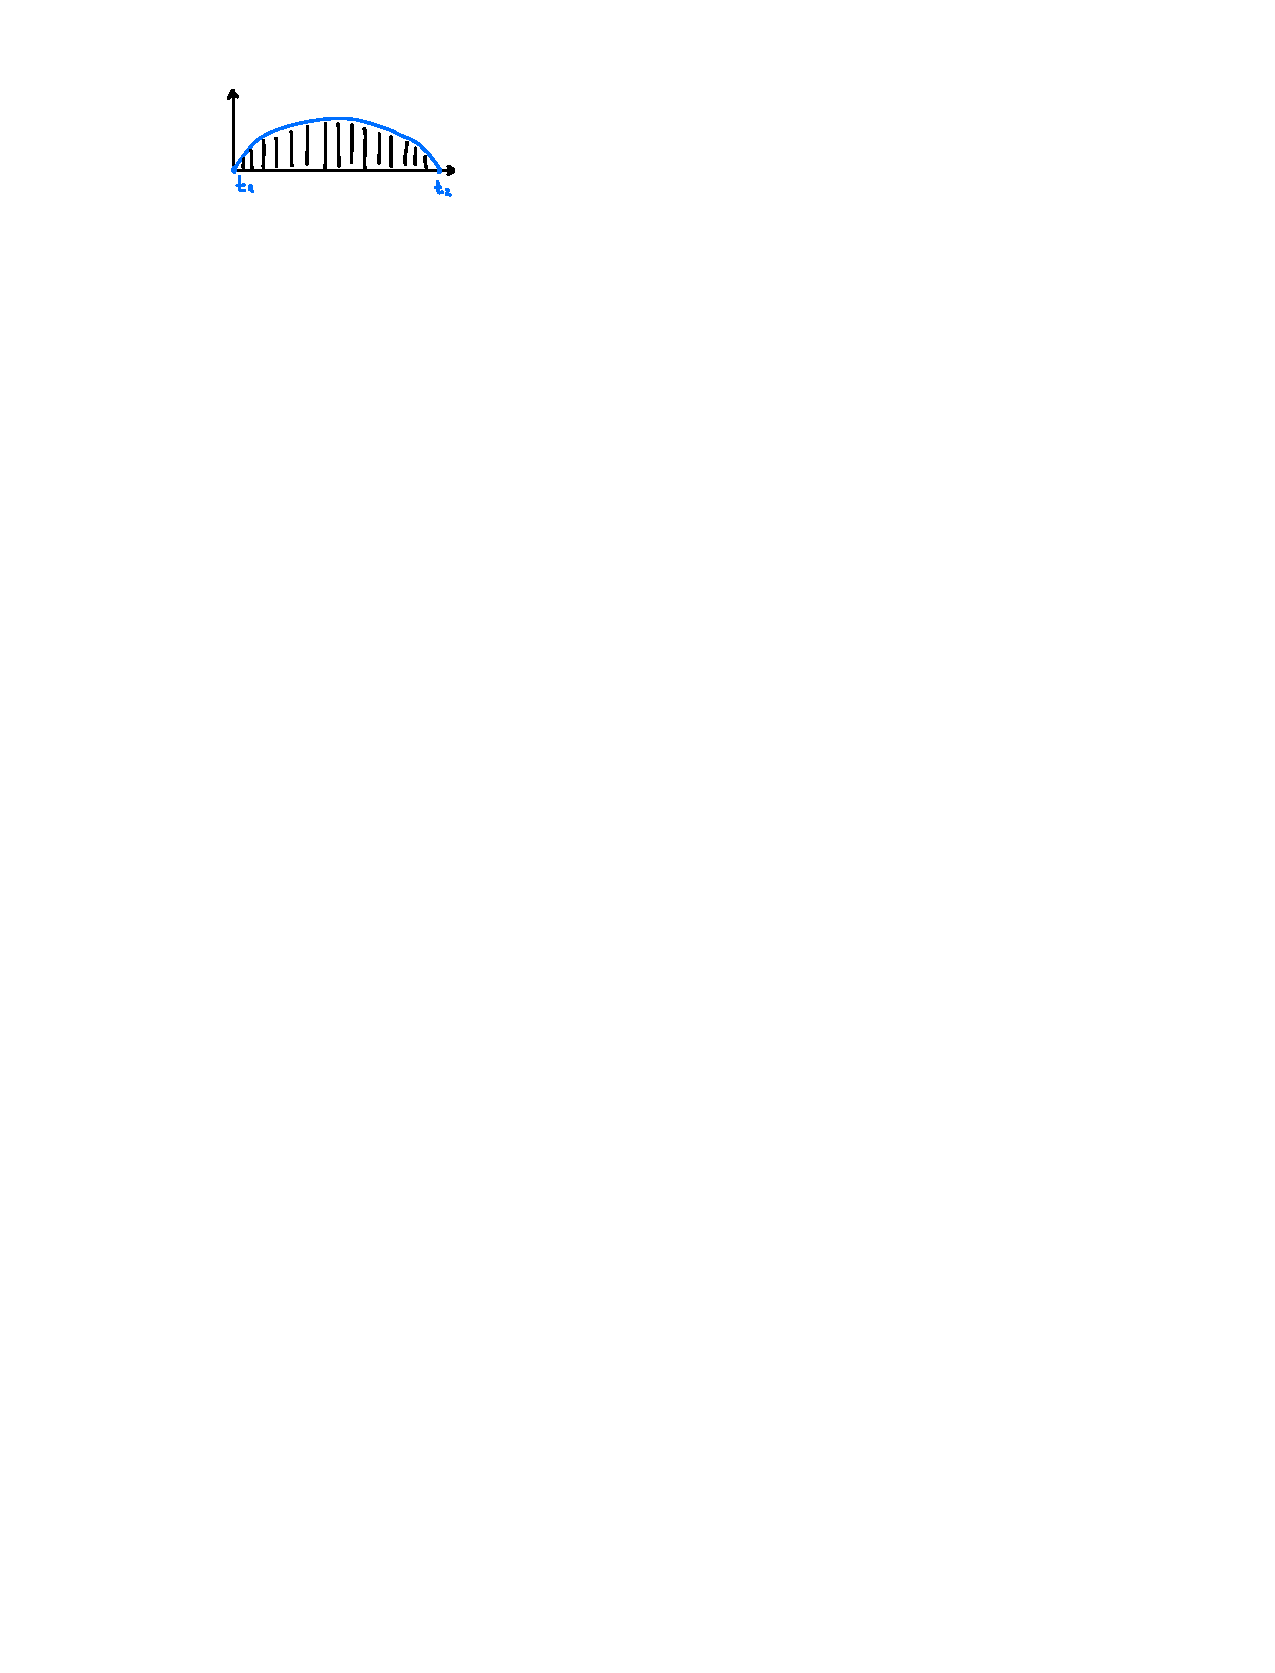
\includegraphics[width=0.7\linewidth]{src/Integralrechnung/param.pdf}
    \end{minipage}

    \subsubsection{Sektorfläche}
        \flushleft Fläche zwischen Ursprung und Kurve
        \begin{minipage}{0.99\linewidth}
            \begin{minipage}{0.65\linewidth}
                \begin{itemize}
                    \item Parametrisierung
                    \item[]  $\displaystyle A= \frac{1}{2} \int_{t_1}^{t_2} (x \dyt - y \dxt) \, dt$   
                    \end{itemize}
            \end{minipage}
            \begin{minipage}{0.34\linewidth}
                    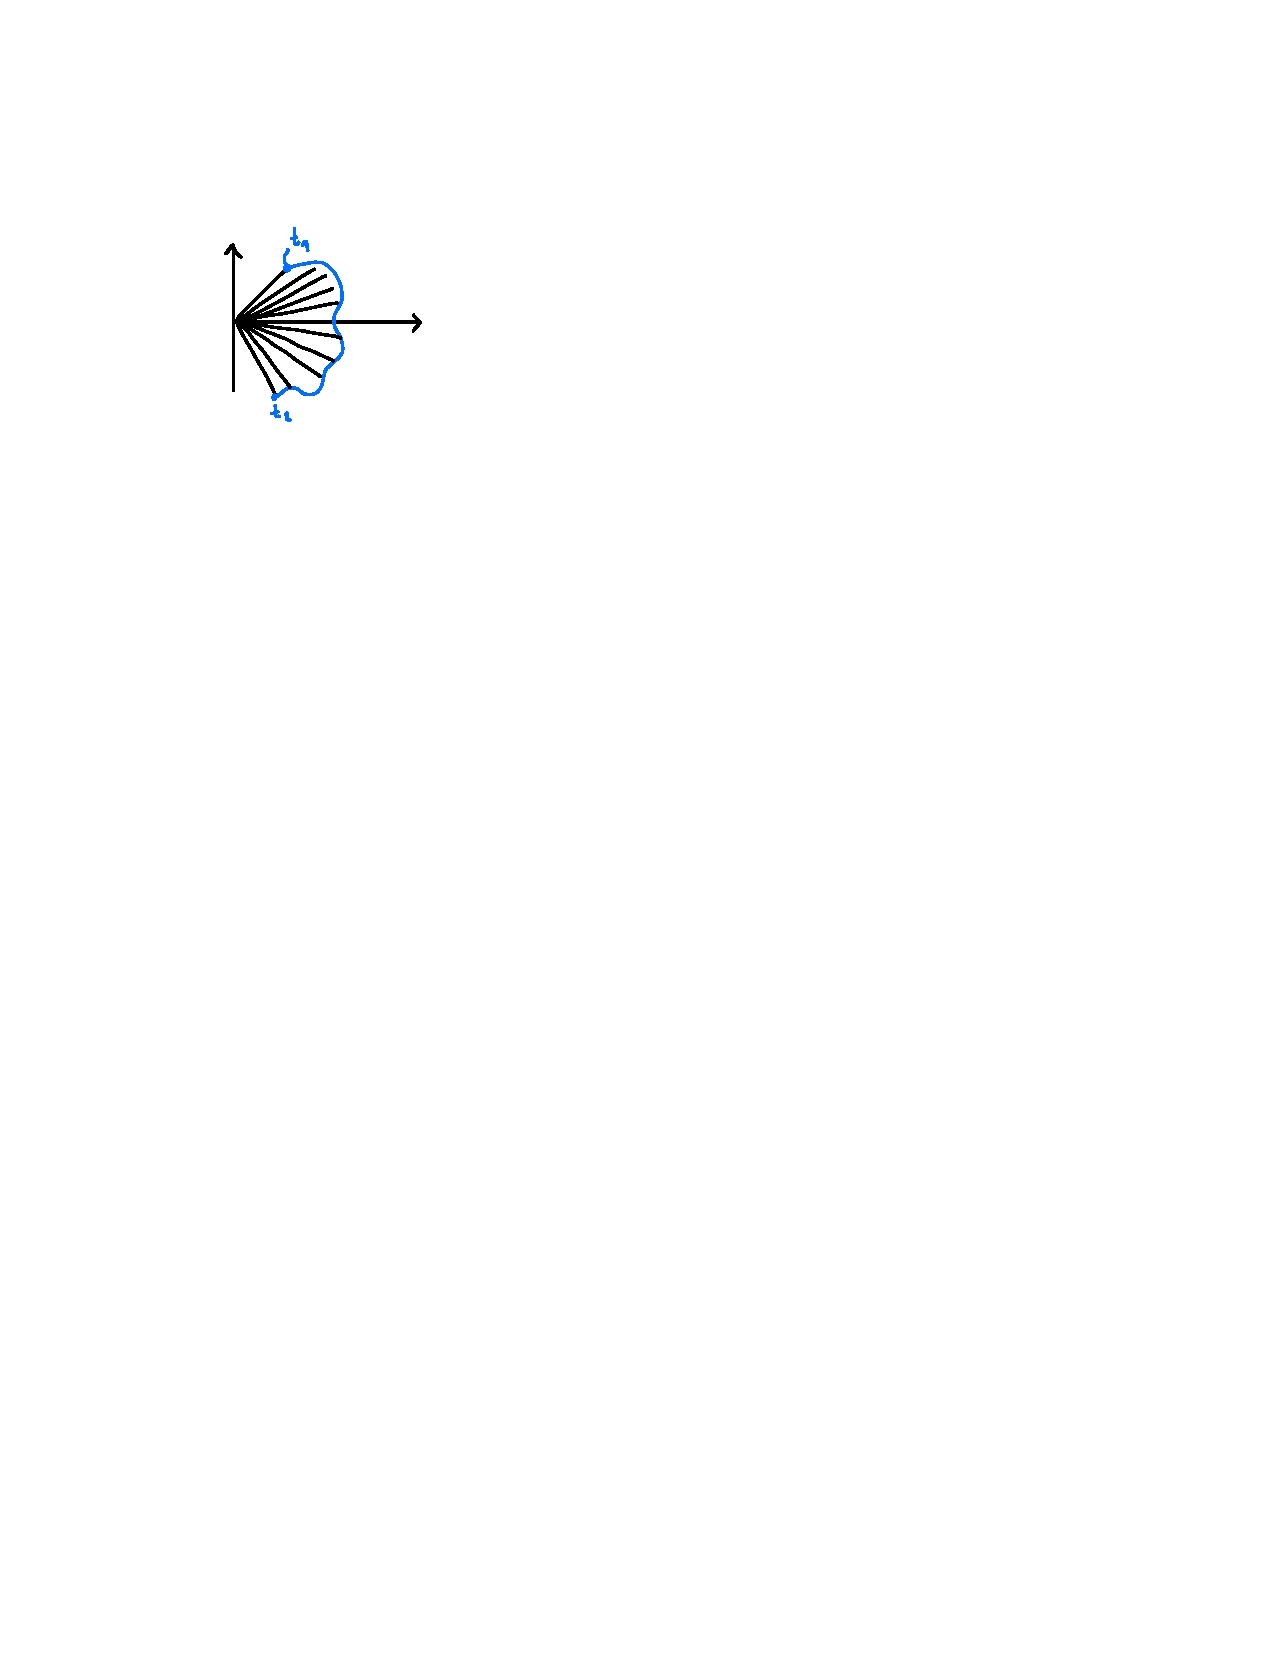
\includegraphics[width=0.6\linewidth]{src/Integralrechnung/sektor.pdf}
            \end{minipage}
        \end{minipage}
        
        \begin{minipage}{0.99\linewidth}
            \begin{minipage}{0.65\linewidth}
                \begin{itemize}
                    \item Polarkoordinaten
                    \item[] $ \displaystyle A= \frac{1}{2} \int_{\varphi_1}^{\varphi_2} \rho^2(\varphi) \, d\varphi $
                \end{itemize}
            \end{minipage}
            \begin{minipage}{0.34\linewidth}
                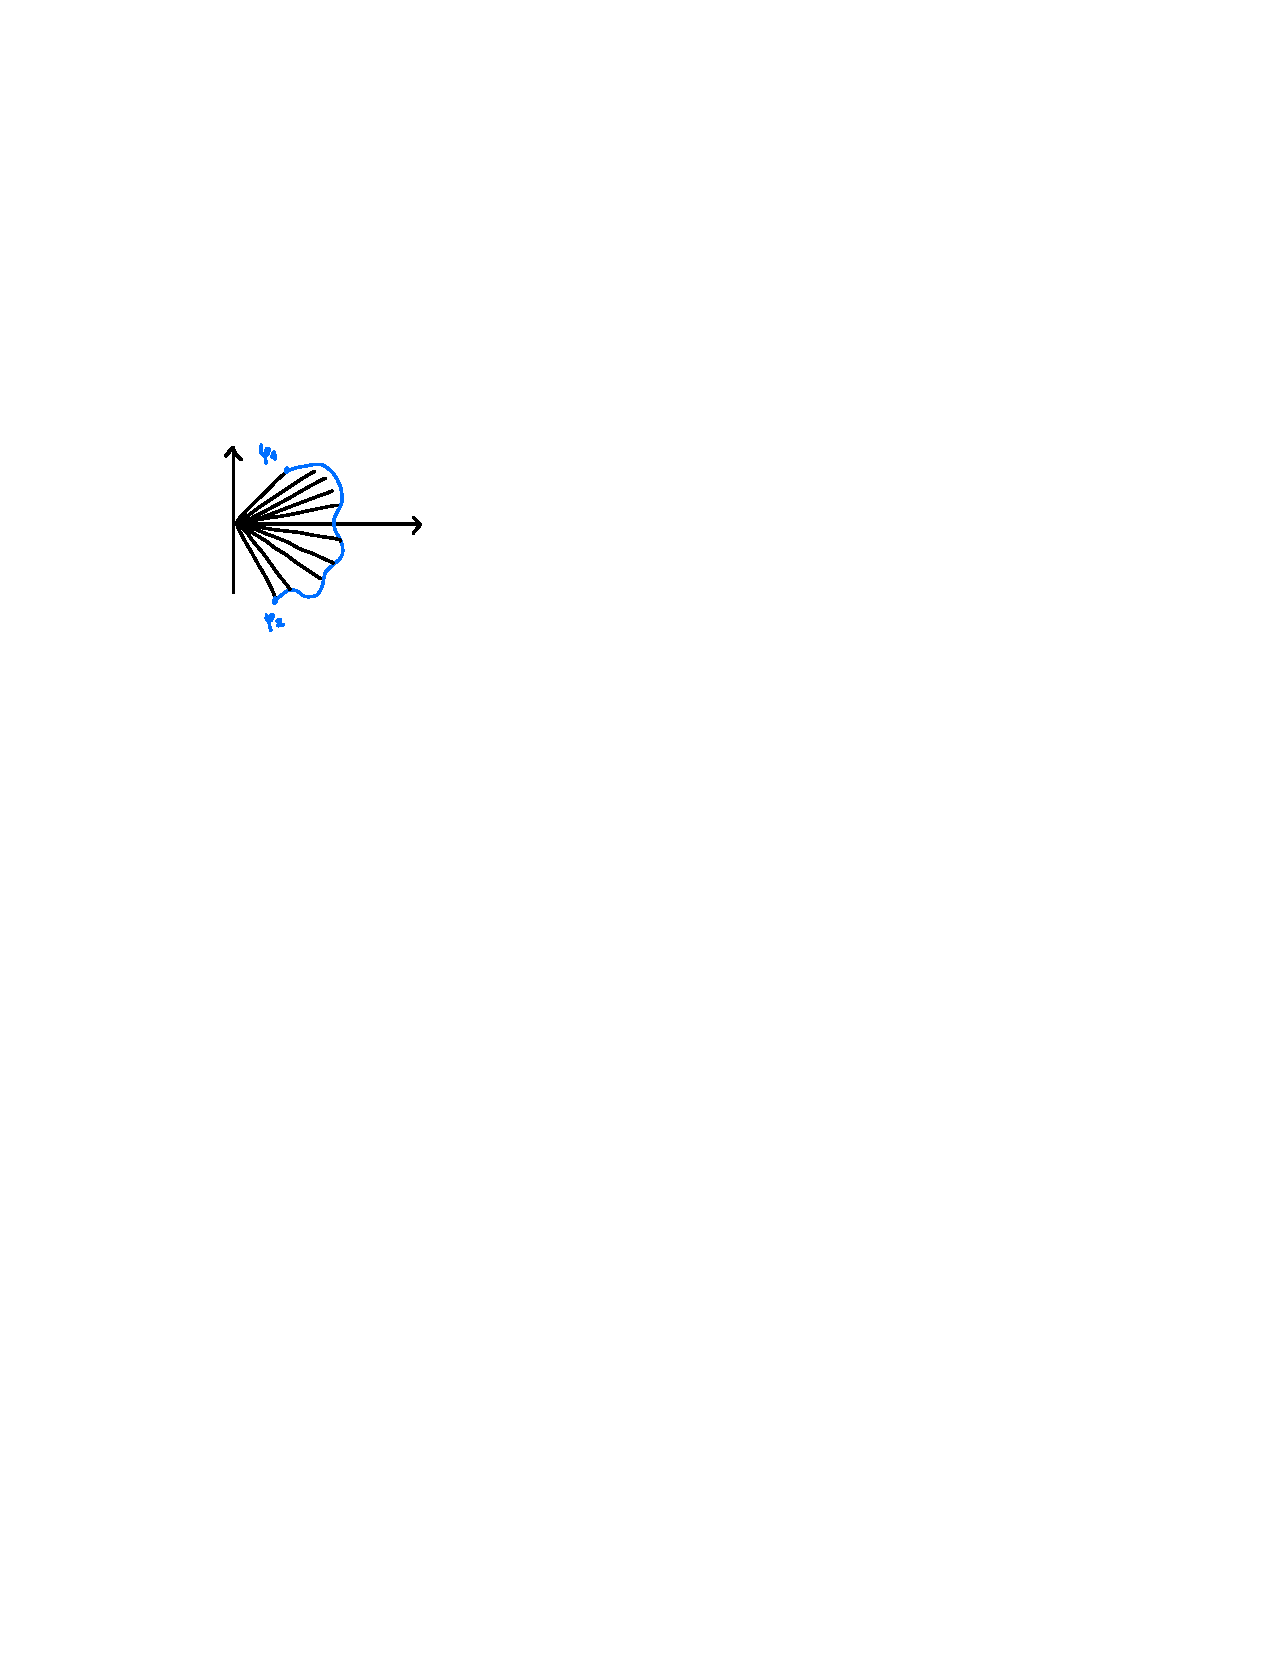
\includegraphics[width=0.6\linewidth]{src/Integralrechnung/polar.pdf}
            \end{minipage}
        \end{minipage}
        {\scriptsize Fläche auf der rechten Seite der Kurve hat positives Vorzeichen.}
        % !TeX root = ../../ZF_bmicha_Ana.tex
\subsection*{Rotationsvolumen}
    \subsubsection*{Kurvenrotation}
        \underline{Kurve rotiert um x-Achse:}
        $$
        V = \int_{t_1}^{t_2} \pi y^2(t) \cdot \underbrace{\dot{x}(t) dt}_{dx} = \int_{x_1}^{x_2} \pi f^2(x) \cdot dx
        $$
        \underline{Kurve rotiert um y-Achse:}
        $$
        V = \int_{t_1}^{t_2} \pi x^2(t) \cdot \underbrace{\dot{y}(t) dt}_{dy} = \int_{y_1}^{y_2} \pi x^2 \cdot \underbrace{f'(x) dx}_{dy}
        $$
    \subsubsection*{Flächenrotation}
        \underline{Fläche unter Kurve rotiert um $y$-Achse:}
        $$
        V = \int_{t_1}^{t_2} \underbrace{2\pi x(t)}_{\textrm{Umfang}} \cdot y(t) \cdot \underbrace{\dot{x}(t) dt}_{dx} = \int_{x_1}^{x_2} 2\pi x \cdot f(x) dx
        $$


        %\vfill \null \columnbreak
        % !TeX root = ../../ZF_bmicha_Ana.tex
\subsection{Rotationsoberflächen}
    \underline{Kurve rotiert um x-Achse:}
    \begin{align*}
        O &= \int_{t_1}^{t_2} 2 \pi y(t) \cdot \underbrace{\sqrt{\dot{x}^2(t) + \dot{y}^2(t)}\ dt}_{ds \textrm{ (Bogenlänge)}}\\
          &= \int_{x_1}^{x_2} 2 \pi f(x) \cdot \underbrace{\sqrt{1 + f'(x)^2}\ dt}_{ds}
    \end{align*}
    \underline{Kurve rotiert um y-Achse:}
    \begin{align*}
        O &= \int_{t_1}^{t_2} 2 \pi x(t) \cdot \underbrace{\sqrt{\dot{x}^2(t) + \dot{y}^2(t)}\ dt}_{ds}\\
          &= \int_{x_1}^{x_2} 2 \pi x \cdot \underbrace{\sqrt{1 + f'(x)^2}\ dx}_{ds}
    \end{align*}

        % !TeX root = ../../ZF_bmicha_Ana.tex
\subsection{Schwerpunkt / Trägheitsmoment}
    Sei $H(x)$ die Höhe des Fläche a.d.S. $x$.\\
    Sei $\sigma$ die Flächendichte $[kg/m^2]$.
    \begin{align*}
        \textrm{Fläche: }  A = \int_{x_1}^{x_2} H(x)\ dx\\
        \textrm{Masse: }  M = \int_{x_1}^{x_2} \sigma \cdot H(x)\ dx\\
        \textrm{Schwerpunkt: }  x_s = \frac{1}{M} \int_{x_1}^{x_2} x \cdot \sigma \cdot H(x)\ dx\\
        \textrm{SP Rotationsvolumen: } x_s = \frac{1}{V} \int_{x_1}^{x_2} x \cdot \pi \cdot H^2(x)\ dx\\
        \textrm{Trägheitsmoment: }  I_y = \int_{x_1}^{x_2} x^2 \cdot \sigma \cdot H(x)\ dx
    \end{align*}
    \subsubsection{Trägheitsmoment}
    \vspace*{-1em}
        \begin{align*}
            \Theta =& \int (\textrm{Abstand zur Rotationsachse})^2 \cdot (\textrm{Masse})\\
            \Theta =& \; \rho \cdot \int_a^b x^2 \cdot G(x) dx\\
            J_0 =& \; \frac{\pi R^4}{2} = \; \parbox{5cm}{polares Flächenträgheitsmoment\\ der Kreisscheibe}\\
            \Theta_x =& \; \rho \cdot \int_a^b \frac{1}{2} \pi (f(x))^4 dx = \; \parbox{5cm}{Masseträgheitsmoment\\ eines Rotationskörpers\\ um die x-Achse}\\
            \Theta =& \; \rho \cdot \frac{1}{2} \pi \int_a^{b} y(t)^4\|\dot{x}(t)\| dt\\
            G(x) =& \; \text{Masse an diesem Abstand}\\
            M(x) =& \; \text{Mantelfäche} = 2 \pi x \cdot G(x) = \text{Umfang} \cdot \text{Höhe}\\ %\underbrace{2 \pi x \vphantom{G(x)}}_{\text{Umfang}} \cdot \underbrace{G(x)}_{\text{Höhe}}\\
            \Theta_z =& \; \rho \int_{x_1}^{x_2} x^2 \cdot M(x) dx
        \end{align*}        
        % !TeX root = ../../ZF_bmicha_Ana.tex
\subsection{Uneigentliche Integrale}
    \begin{center}
        Konvergiert $\Longleftrightarrow$ Grenzwert existiert
    \end{center}
    
    \subsubsubsection{1. Gattung}
            Zu integrierende Funktion ist an der Grenze nicht definiert. Bsp.:
            $$
                \int\limits_{0}^{1}  \frac{1}{x} \ dx = \lim_{\xi \to 0^+} \int\limits_{\xi}^{1} \frac{1}{x} \ dx
            $$
    \subsubsubsection{2. Gattung}
        Unendlicher Integrationsbereich. Bsp.:
        $$
            \int\limits_{0}^{\infty}  f(x) \ dx = \lim_{\xi \to \infty}\int\limits_{0}^{\xi} f(x) \ dx
        $$
    \subsubsection{Tricks}
        \vspace{-0.5em}
        \begin{align*}
            \int\limits_{1}^{\infty}  \frac{1}{x^\alpha} \ dx  \qquad &\text{konvergiert} \iff \alpha > 1\\
            \int\limits_{0}^{1}  \frac{1}{x^\alpha} \ dx  \qquad &\text{konvergiert} \iff \alpha < 1  
        \end{align*}
    \section{Potenzreihen \texorpdfstring{\hfill FoTaBe S.77}{ - FoTaBe S.77}}
        % !TeX root = ../../ZF_bmicha_Ana.tex
Potenzreihe der Funktion $f(x)$ um den Punkt $x_o$:
\mathbox{
    f(x) = \sum_{n=0}^{\infty} a_n \cdot (x-x_o)^n
}
\begin{itemize}
    \item Höchstens eine Potenzreihe von $f$ um $x_o$ existiert.
    \item Konvergiert für $\abs*{x-x_o} < r$
\end{itemize}
\mathbox{
    \frac{1}{1 - \fcolorbox{green}{white}{x}} = \sum\limits_{n = 0}^{\infty} \fcolorbox{green}{white}{x}^k
}
        % !TeX root = ../../ZF_bmicha_Ana.tex
\subsection{Konvergenzradius}
    \vspace{0.5em}
    \mathbox{
        r = \lim_{n\to\infty} \left\lvert \frac{a_n}{a_{n+1}} \right\rvert
    }
    \begin{center}
            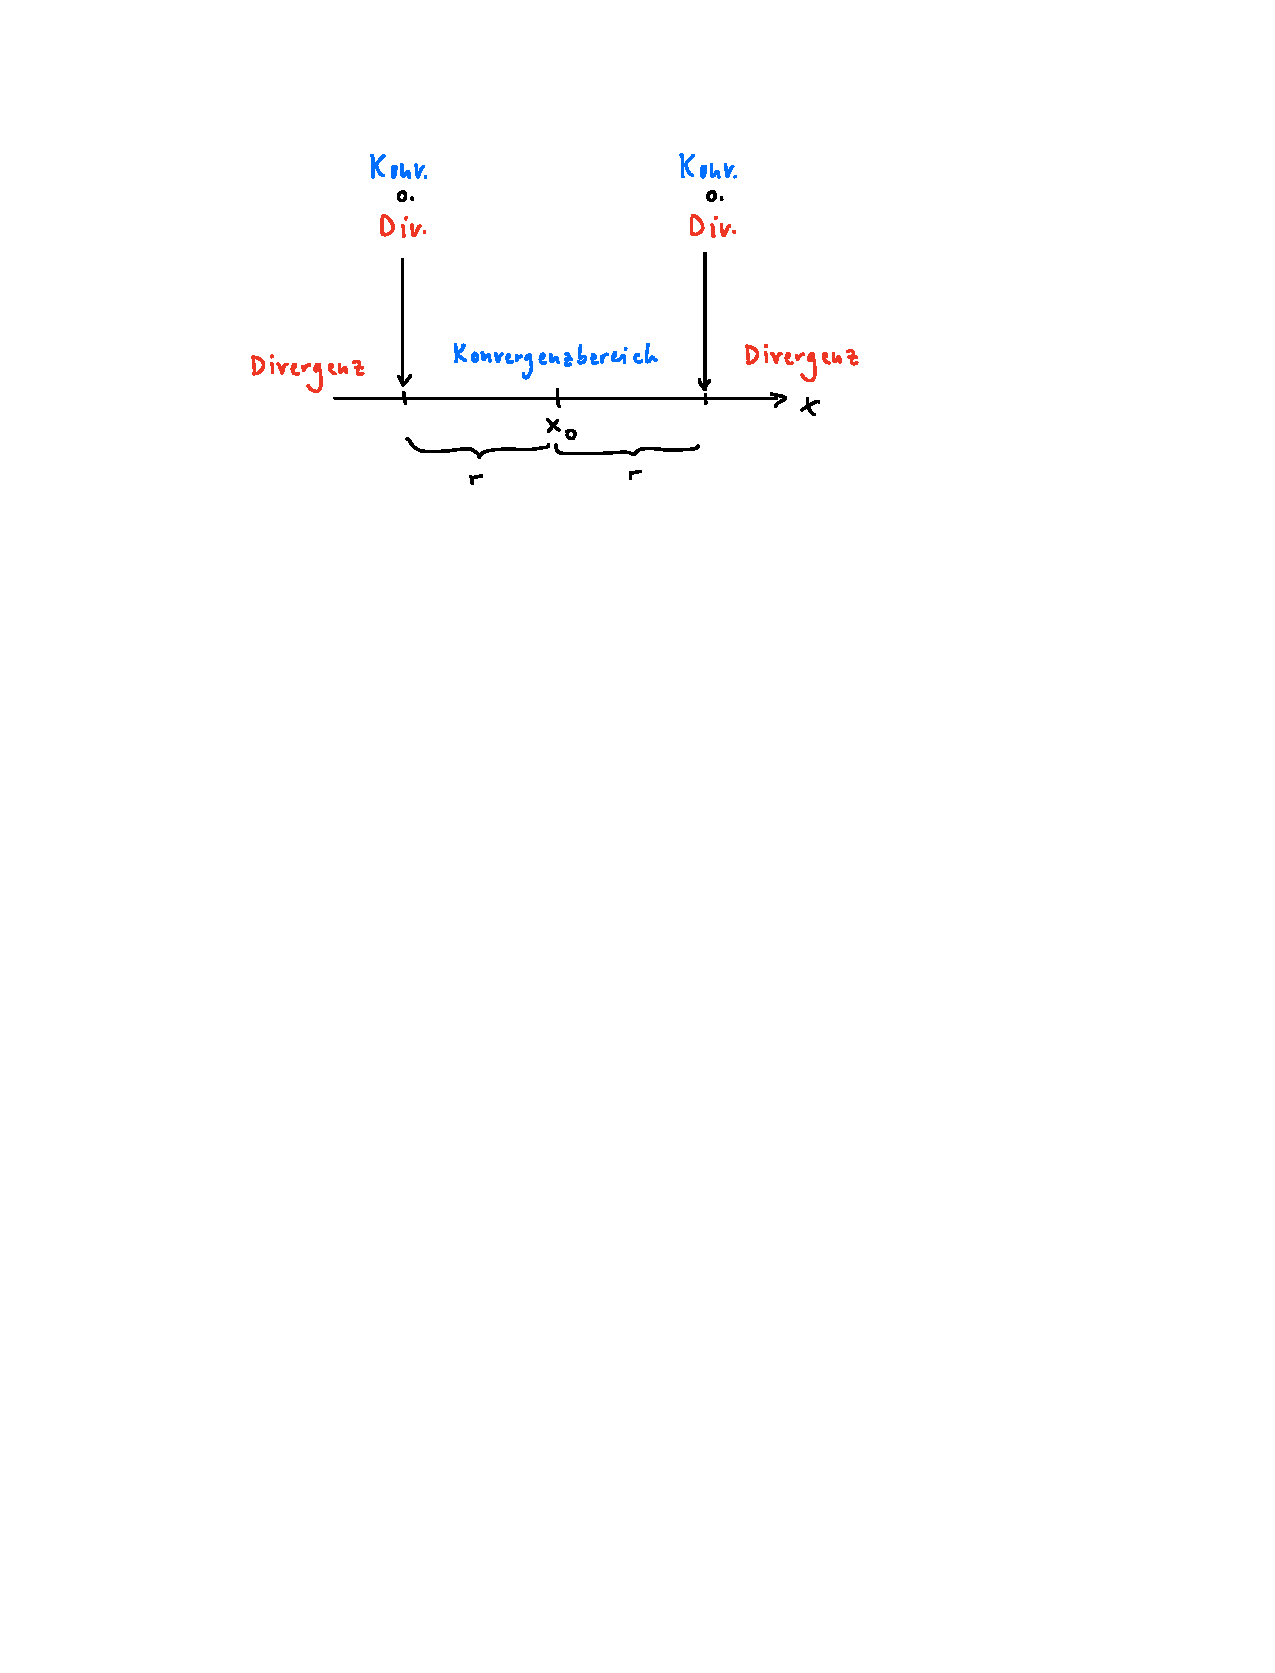
\includegraphics[width=0.65\linewidth]{src/Potenzreihen/konvergenzradius.pdf}
    \end{center}
    Innerhalb vom Konvergenzbereich darf man Potenzreihen \textit{gliedweise}:
    \begin{itemize}
        \item addieren \& subtrahieren
        \item integrieren \& differenzieren
    \end{itemize}
        % !TeX root = ../../ZF_bmicha_Ana.tex
\subsection{Taylorreihen}
    Taylorentwicklung von $f(x)$ um $x_o$:
    \mathbox{
        f(x) = \sum_{n=0}^\infty \frac{f^{(n)}(x_o)}{n!} (x-x_o)^n
    }
    \begin{itemize}
    \item ungerade Fkt $\Leftrightarrow$ ungerade Indizes: $a_1x + a_3x^3 + \dots$
    \item gerade Fkt $\Leftrightarrow$ gerade Indizes: $a_0 + a_2x^2 + \dots$
    \end{itemize}
        \vfill \null \columnbreak
    \section{Trigonometrie}
        \subsection{Werte Tabelle}
    \begin{center}
        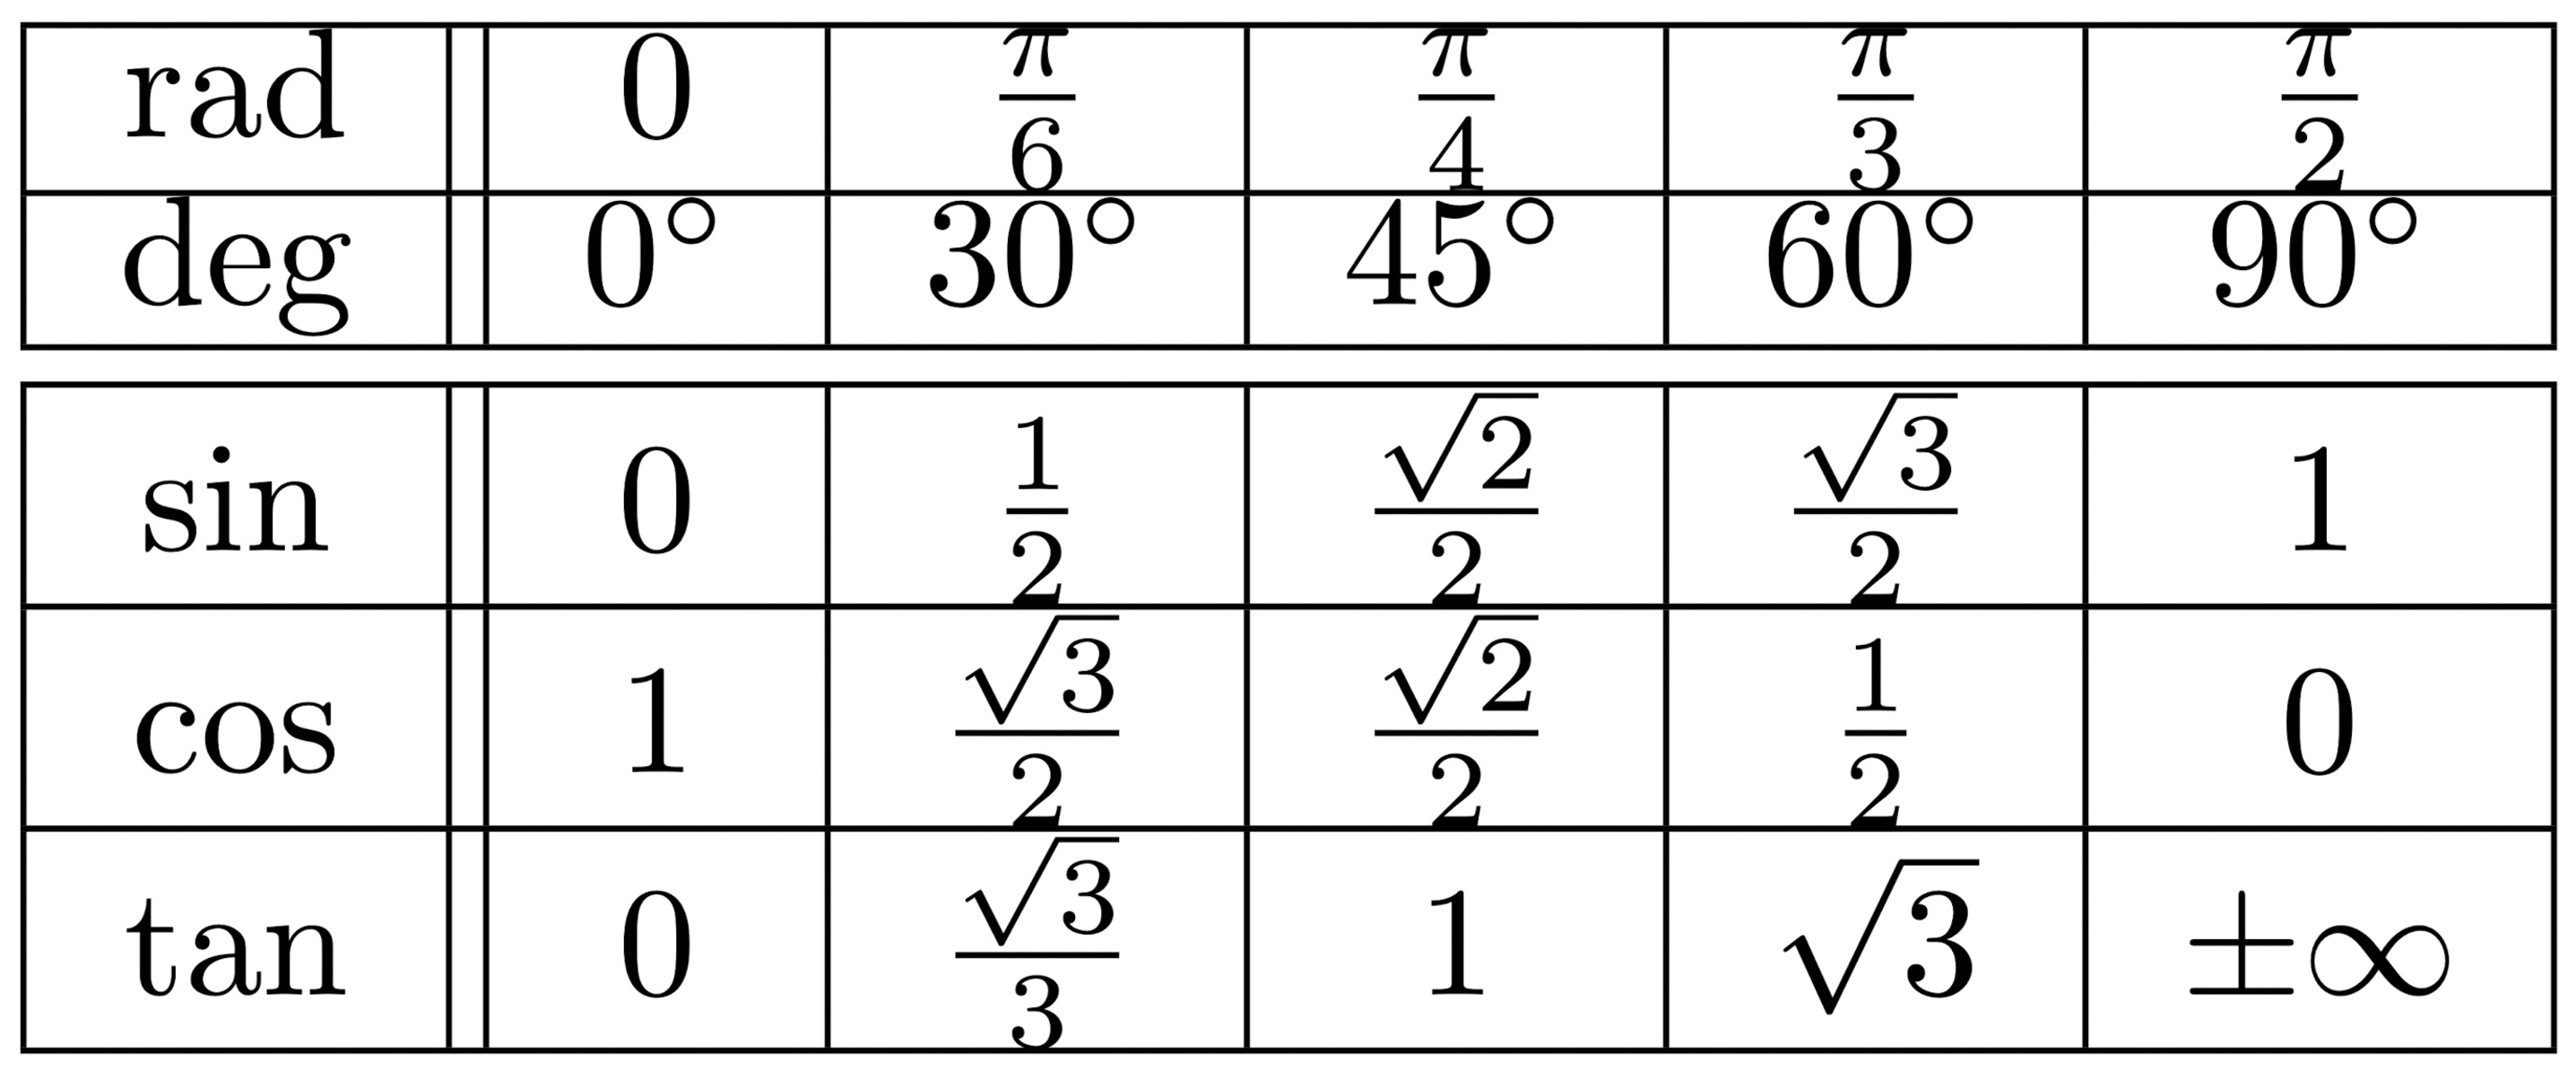
\includegraphics[width=0.7\linewidth]{src/Trigonometrie/trigo_tabelle.pdf}
    \end{center}
        % \subsection{Einheitskreis}
    \centerline{
        \resizebox{4cm}{4cm}{
            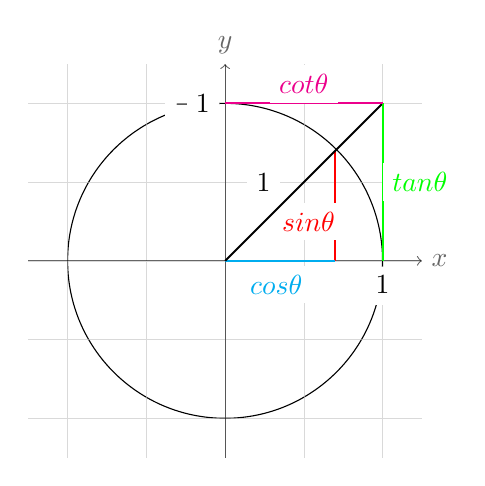
\begin{tikzpicture}
                %circle
                \draw[smooth, samples = 600] (0, 0) circle (2)(1, 1);
                
                % coordinate system
                \draw[opacity=0.6,lightgray,very thin,step=1cm](-2.5,-2.5) grid (2.5,2.5);
                \draw[->,opacity=0.6](-2.5,0) -- (2.5,0) node [right]{$x$};
                \foreach \x in {-1,...,1}
                \draw[xshift=2cm] (0,2pt) -- (0,-2pt) node[below,fill=white]{$\x$};
                \draw[->,opacity=0.6](0,-2.5) -- (0,2.5) node[above]{$y$};
                \foreach \y in {-1,...,1}
                \draw[yshift=2cm] (2pt,0) -- (-2pt,0) node[left,fill=white] {$\y$};
                
                %sin
                \draw[line width=0.25mm,red] (1.39, 1.39) -- (1.39,0);
                    \draw (0.6,0.5) node[red,right,fill=white] {$sin\theta$};
                %cos
                \draw[line width=0.25mm,cyan] (0, 0) -- (1.39, 0);
                    \draw (0.65,-0.3) node[cyan,fill=white] {$cos\theta$};
                %Hypotenuse
                \draw[line width=0.25mm,black] (0, 0) -- (2, 2);
                    \draw (0.7,1) node[left, black,fill=white] {$1$};
                %tan
                \draw[line width=0.25mm,green] (2,0) -- (2, 2);
                    \draw (2, 1) node[green, right, fill=white] {$tan\theta$};
                %cot
                \draw[line width=0.25mm,magenta] (2, 2) -- (0, 2);
                    \draw (1, 2) node[magenta, above, fill=white] {$cot\theta$};
                
            \end{tikzpicture}
        }
    }
    \vspace*{0.5em}
        \subsection{Rechenregeln}
\vspace*{-1em}
    \begin{align*}
        1 =& \; sin(x)^2 + cos(x)^2\\
        \sin(\alpha \pm \beta) =& \; \sin \alpha \cos \beta \pm \cos \alpha \sin \beta\\
        \sin(2 \alpha) =& \; 2 \sin \alpha cos \alpha\\
        \sin(3 \alpha) =& \; 3 \sin \alpha - 4 sin^3 \alpha\\
        \sin^2 \frac{\alpha}{2} =& \; \frac{1 - \cos \alpha}{2}\\
        \cos(\alpha \pm \beta) =& \; \cos \alpha \cos \beta \mp \sin \alpha \sin \beta\\
        \cos(2 \alpha) =& \; \cos^2 \alpha - \sin^2 \alpha\\
        =& \; 2 \cos^2 \alpha - 1 = 1 - 2 \sin^2 \alpha\\
        \cos(3 \alpha) =& \; 4 \cos^3 \alpha - 3 \cos \alpha\\
        cos^2 \frac{\alpha}{2} =& \; \frac{1 + cos \alpha}{2}\\
        \frac{a}{sin(\alpha)} =& \; \frac{b}{sin(\beta)} = \frac{c}{sin(\gamma)}\\
        a^2 =& \; b^2 + c^2 - 2bc \cdot cos(\alpha)
    \end{align*}


        \subsection{Funktionsmodifikation}
\vspace*{-1em}
    \begin{align*}
        \text{Frequenz} \; f: t \rightarrow& \; \sin(\frac{2 \pi}{T} t)\\
        \text{Amplitude} \; f: t \rightarrow& \; A \cdot \sin(t)\\
        \text{Winkelgeschwindigkeit} \; \omega =& \; \frac{2 \pi}{T} \left[\frac{1}{s}\right]
    \end{align*}
    % \cbreak
    % \section{Mehrdimensionale Fkt. - Diff. Rechnung}
        % % !TeX root = ../../ZF_bmicha_Ana.tex
\subsection{Allgemeine Fehlerrechnung}
    Die berechnete Grösse $f$ ist abhängig von den gemessenen Grössen $x,y$.
    Die gemessenen Grössen weichen mit den Messfehlern $dx,dy$ von der Realität ab.
    \begin{itemize}
        \item \textbf{Totales Differential / Absoluter Fehler}
            \mathbox{
                df \approx f_x\ dx + f_y\ dy
            }
        \item \textbf{Relativer Fehler}
            \mathbox{
                \frac{df}{f}
            }
    \end{itemize}
    %     % !TeX root = ../../ZF_bmicha_Ana.tex
\subsection{Niveaulinien / -flächen}
    \vspace{0.5em}
    \begin{minipage}{0.4\linewidth}
        \begin{center}
            \underline{\textbf{2D}}
        \end{center}
        $$
            f(x,y) = C , \quad C \in \mathbb{R}
        $$
        \begin{center}
            \textit{Höhenlinien}
        \end{center}
    \end{minipage}
    \hspace{0.05\linewidth}
    \begin{minipage}{0.5\linewidth}
        \begin{center}
            \underline{\textbf{3D}}
        \end{center}
        $$
            f(x,y,z) = C , \quad C \in \mathbb{R}
        $$
        \begin{center}
            \textit{Flächen mit konst. Temp.}
        \end{center}
    \end{minipage}
    %     % !TeX root = ../../ZF_bmicha_Ana.tex
\subsection{Gradient}
    \vspace{-0.75em}
    $$
        \grad(f(x,y,z)) = 
        \begin{pmatrix}
            f_x \\ f_y \\ f_z
        \end{pmatrix}
        =
        \begin{pmatrix}
            \frac{\partial}{\partial x} \\[0.4em] \frac{\partial}{\partial y} \\[0.4em] \frac{\partial}{\partial z}
        \end{pmatrix}
    $$
    \begin{itemize}
        \item Steht senkrecht auf Niveauflächen/ -linien.
        \item Zeigt in Richtung des grössten Anstiegs der Funktionswerte.
    \end{itemize}
    \vspace*{0.5em}
    \subsubsection{2D - $f(x,y)$}
        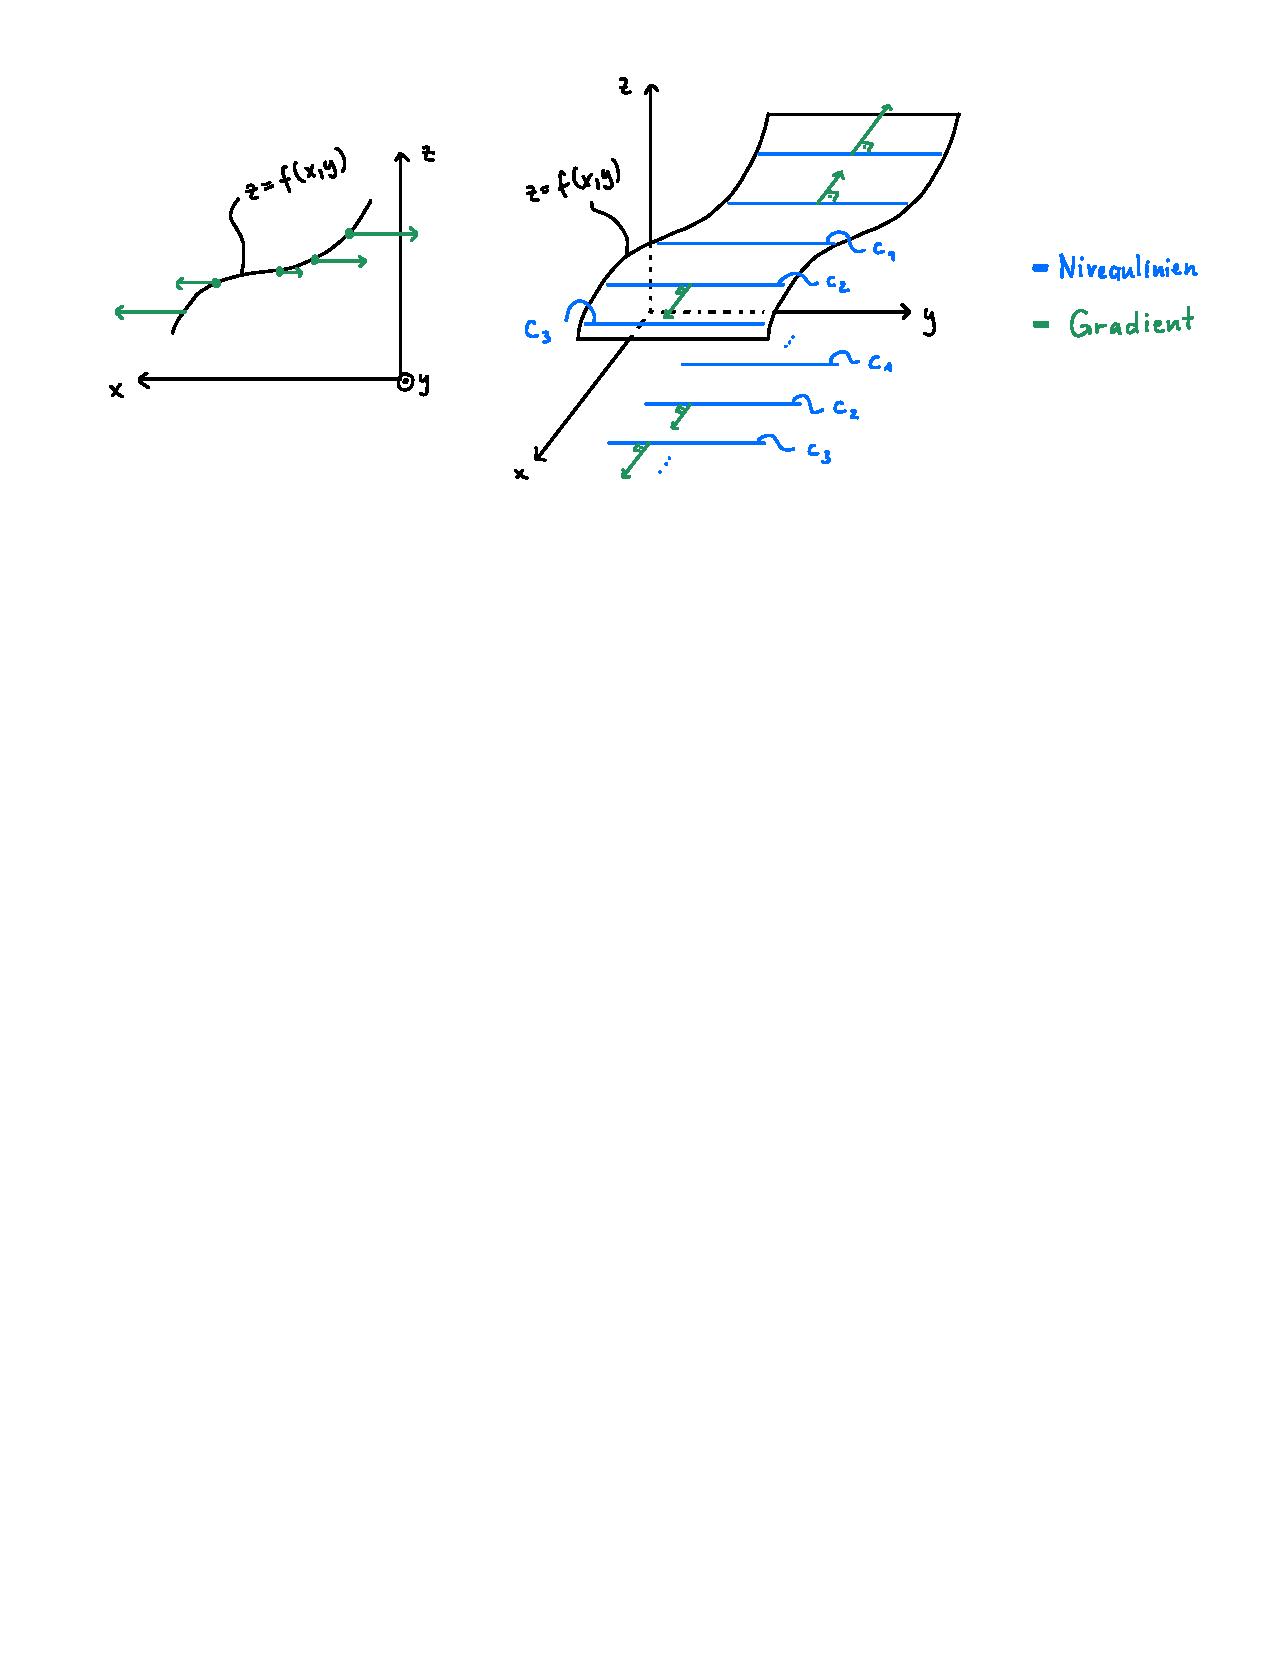
\includegraphics[width=\linewidth]{src/Mehrdimensionale-Funktionen_Differentialrechnung/grad_2D.pdf}
    \subsubsection{3D - $f(x,y,z)$}
        \begin{center}
            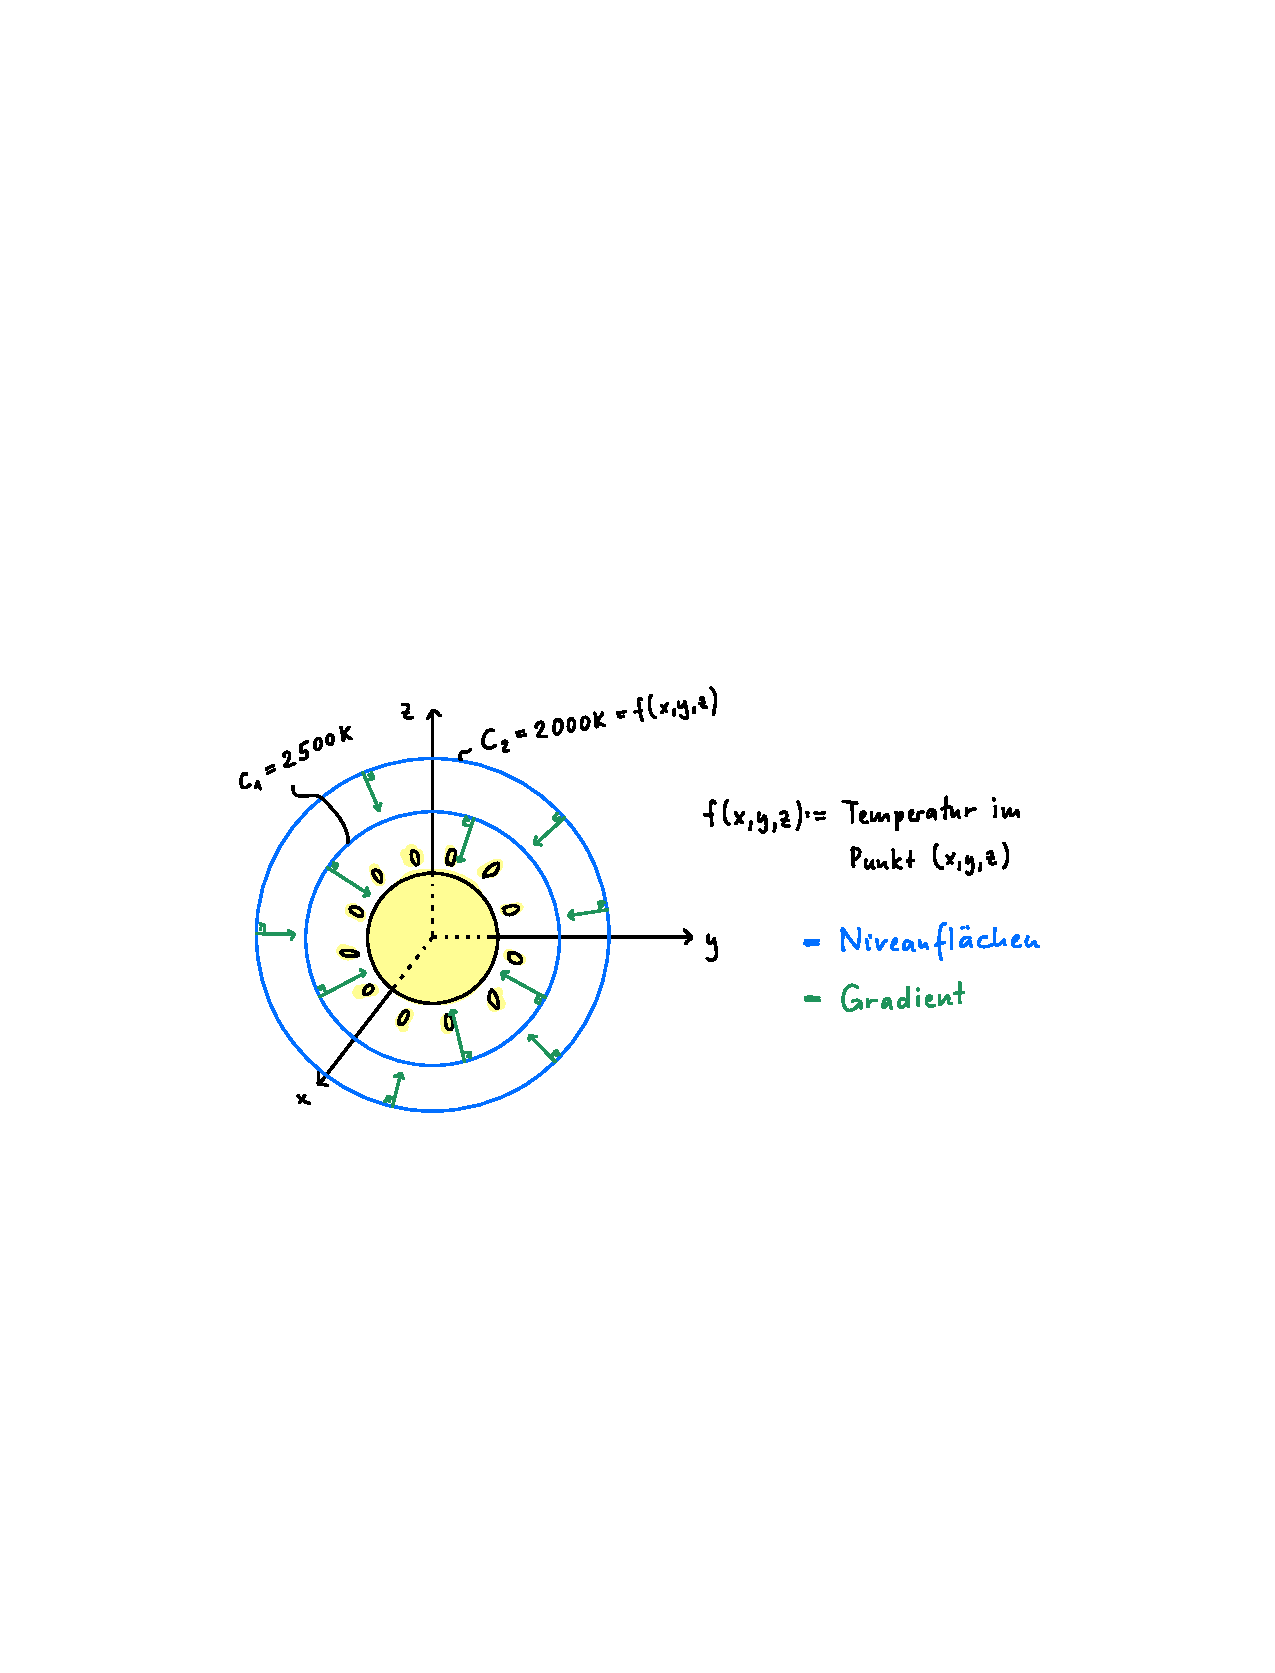
\includegraphics[width=0.8\linewidth]{src/Mehrdimensionale-Funktionen_Differentialrechnung/grad_3D.pdf}
        \end{center}
    %     % !TeX root = ../../ZF_bmicha_Ana.tex
\subsection{Richtungsableitung}
    Steigung von $f$ in Richtung $\vec{e}$ im Punkt $\vec{r}_o$:
    $$
        D_{\vec{e}f} = \frac{\vec{e}}{ \lvert\vec{e}\,\rvert} \cdot \textrm{grad} f (\vec{r}_o)
    $$
    %     % !TeX root = ../../ZF_bmicha_Ana.tex
\subsection{Tangentialebenen}
    \subsubsection{Linearisierungsformel}
        \vspace{0.5em}
        \mathbox{
            z = f(x_o,y_o) + f_x(x_o,y_o) (x\!-\!x_o) + f_y(x_o,y_o)(y\!-\!y_o)
        }
        \mathbox{
            0 = f_x(x_o,y_o,z_o)(x\!-\!x_o) + f_y(x_o,y_o,z_o)(y\!-\!y_o) + \dots
        }
    \subsubsection{Gradient}
        \begin{itemize}
            \item $f(x,y,z) = C$ ist eine Niveaufläche
            \item $\grad(f)$ steht senkrecht auf Niveauflächen. ($\to \nvec$ )
            \item Ebene mit Normalenvektor $\nvec = (A,B,C)^T$:
            $$
                Ax + By + Cz = D
            $$
        \end{itemize}
    %     % !TeX root = ../../ZF_bmicha_Ana.tex
\subsection{Extremalstellen von $f(x,y)$}
    \vspace{0.25em}
    \begin{enumerate}
        \item Inneres untersuchen $\to$ $\textrm{grad}f \overset{!}{=} 0$
        \item Rand untersuchen
        \begin{itemize}
            \item Lagrange Multiplikatoren
            \begin{enumerate}
                \item $g(x,y)$ beschreibt Rand
                \item $\textrm{grad}f(x_o,y_o) = \lambda \cdot \textrm{grad}\, g(x_o,y_o)$\\[0.25em]
                      \phantom{llll}$\textrm{grad}\, g(x_o,y_o) \neq 0,\phantom{ll} \lambda \in \mathbb{R}$
                \item Gleichungssystem aus (a) und (b) lösen.
            \end{enumerate}
            \item Parametrisierung
            \begin{enumerate}
                \item Rand parametrisieren
                \item Parametrisierung in $f$ einsetzen
                \item Nach Parameter ableiten und nullsetzen.\\[0.25em] \phantom{llll}$f'(t) = 0$
            \end{enumerate}
        \end{itemize}
        \item Eckpunkte untersuchen
        \item Kandidaten vergleichen
    \end{enumerate}
    %     \subsection{Satz von Schwarz}
    \textit{Reihenfolge von partiellen Ableitungen einer stetigen Funktion spielt keine Rolle:  $f_{xxyyzz} = f_{xzyxyz}$}
    % $$
    %     f_{xxyyzz} = f_{xzyxyz}
    % $$
    % \vspace{-1em}
    % \cbreak
    %     \subsection{Integrabilitätsbedingungen (IB)}
    Geg.: $\phi(x,y), \psi(x,y)$\\[0.25em]
    Ges.: $f(x,y)$ mit:
    \begin{align*}
        f_x \equiv \phi \quad \textrm{und} \quad f_y \equiv \psi
    \end{align*}
    \begin{enumerate}
        \item IB prüfen (Satz von Schwarz):
            $$ \phi_y \equiv \psi_x$$
        \item $f(x,y)$ bestimmen (Konstante nicht vergessen!):
            $$ f = \int \phi\, dx = \int \psi\, dy $$
    \end{enumerate}
    \vspace*{-0.5em}
    %     % !TeX root = ../../ZF_bmicha_Ana.tex
\subsection{Verallgemeinerte Kettenregel}
    \vspace{-0.5em}
    $$
        Geg.: f(x,y,z),\quad x(t), y(t), z(\rho),\quad \rho(t)
    $$
    \vspace{0.25em}
    $$
        \frac{df}{dt} = \frac{\partial f}{\partial x}   \frac{dx}{dt} + \frac{\partial f}{\partial y} \frac{dy}{dt} + \frac{\partial f}{\partial z} \frac{dz}{d\rho} \frac{d\rho}{dt}
    $$
    % \section{Mehrdimensionale Fkt. - Int. Rechnung}
    %     % !TeX root = ../../ZF_bmicha_Ana.tex
\subsection{Flächen- \& Volumenintegrale}
    \vspace{0.5em}
    \begin{minipage}{0.4\linewidth}
        \begin{center}
            \underline{\textbf{2D}}
        \end{center}
        $$
            \iint f(x,y) \,\, dA
        $$
        \begin{center}
            \textit{Flächenintegral}
        \end{center}
    \end{minipage}
    \hspace{0.05\linewidth}
    \begin{minipage}{0.5\linewidth}
        \begin{center}
            \underline{\textbf{3D}}
        \end{center}
        $$
           \iiint f(x,y,z) \,\, dV
        $$
        \begin{center}
            \textit{Volumenintegral}
        \end{center}
    \end{minipage}
    %     % !TeX root = ../../ZF_bmicha_Ana.tex
\subsection{Dimensionsvergleich}
    \vspace{-1.25em}
    \begin{align*}
        \int f(x)\, dx &= Fl\ddot{a}che = \iint 1\, dA\\ % dirty hack is dirty
        \iint f(x,y)\, dA &= Volumen = \iiint 1\, dV\\
        \iiint f(x,y,z)\, dV &= ...
    \end{align*}
    \vspace{-0.75em}
    %     % !TeX root = ../../ZF_bmicha_Ana.tex
\subsection{Koordinatentransformationen}
    \begin{center}
        \textit{kartesisch:}
    \end{center}
    \begin{minipage}{0.49\linewidth}\vspace{-1em}
        \begin{align*}
            dA = dxdy \phantom{ml}
        \end{align*}
    \end{minipage}
    \begin{minipage}{0.49\linewidth}\vspace{-1em}
        \begin{align*}
            dV = dxdydz \phantom{ll}
        \end{align*}
    \end{minipage}

    \hrule
    \begin{center}
        \textit{zylindrisch:}
    \end{center}\vspace{-0.25em}
    \begin{minipage}{0.49\linewidth}\vspace{-1em}
        \begin{align*}
            x &= r \cos(\varphi)\\
            y &= r \sin(\varphi)\\\\[0.25em]
            dA &= r \, drd\varphi
        \end{align*}
    \end{minipage}
    \begin{minipage}{0.49\linewidth}\vspace{-1em}
        \begin{align*}
            x &= r \cos(\varphi)\\
            y &= r \sin(\varphi)\\
            z &= z\\[0.25em]
            dV &= r \, drd\varphi dz
        \end{align*}
    \end{minipage}\vspace{0.5em}

    \hrule
    \begin{center}
        \textit{sphärisch:}
    \end{center}\vspace{-0.25em}
    \begin{center}
        \begin{minipage}{0.49\linewidth}\vspace{-1em}
            \begin{align*}
                x &= r \sin(\theta)\cos(\varphi)\\
                y &= r \sin(\theta)\sin(\varphi)\\
                z &= r \cos(\theta)\\[0.25em]
                dV &= r^2 \sin(\theta) \, drd\varphi d\theta
            \end{align*}
        \end{minipage}
    \end{center}
    %     % !TeX root = ../../ZF_bmicha_Ana.tex
\subsubsection{Ellipsenkoordinaten}
    \begin{minipage}{0.49\linewidth}
        \vspace{0.5em}
        \underline{\textbf{Rand:}}\\
        \textit{implizit:}
        $$
            \left( \frac{x}{a} \right)^2 + \left( \frac{y}{b} \right)^2 = 1
        $$
        \textit{parametrisiert:}
        \begin{align*}
            x &= a \cdot \cos(\varphi)\\
            y &= b \cdot \sin(\varphi)\\
        \end{align*}
    \end{minipage}
    \begin{minipage}{0.5\linewidth}
        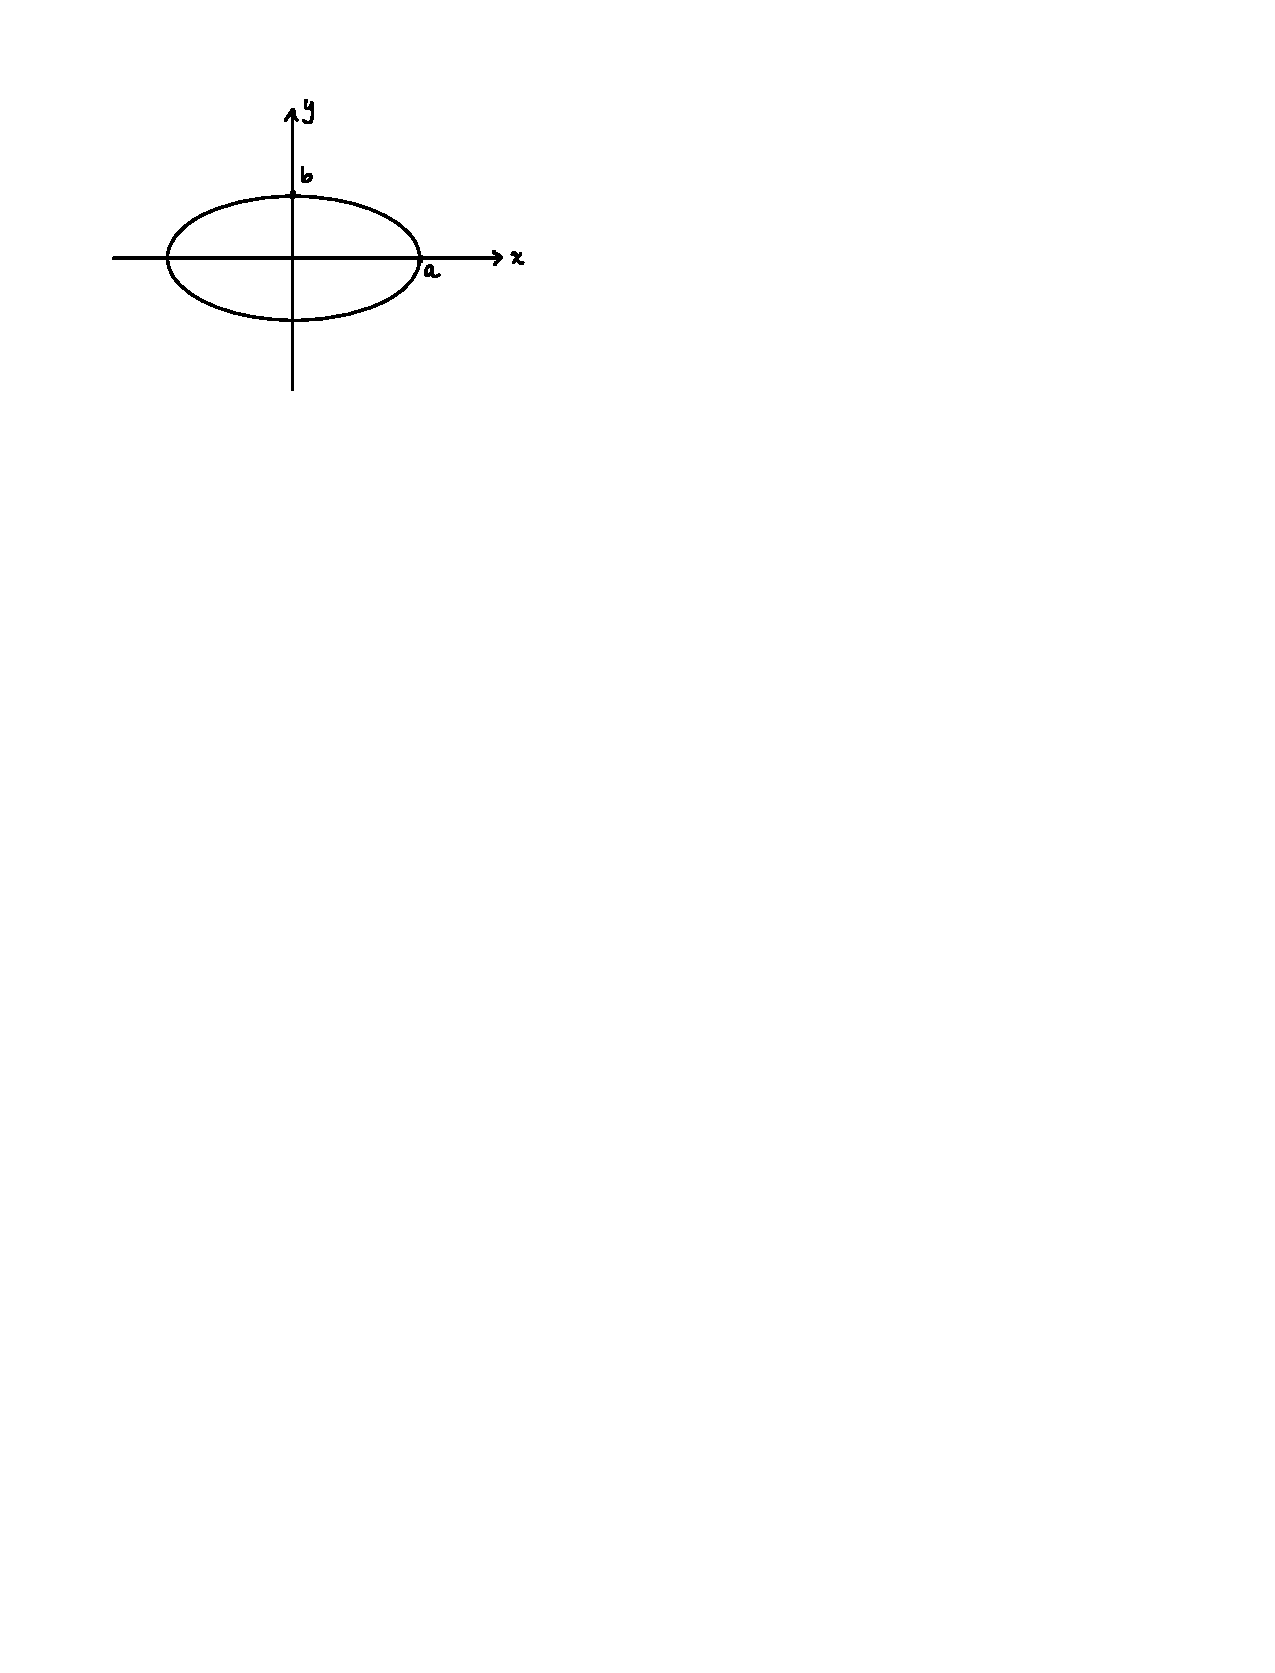
\includegraphics[width=\linewidth]{src/Mehrdimensionale-Funktionen_Integralrechnung/ellipse.pdf}
    \end{minipage}\vspace{-1em}
    \begin{minipage}{0.49\linewidth}
        \textbf{\underline{Fläche:}}
            \begin{align*}
                x &= a \cdot r \cdot \cos(\varphi)\\
                y &= b \cdot r \cdot \sin(\varphi)
            \end{align*}
    \end{minipage}
    \begin{minipage}{0.5\linewidth}
        \vspace{0.8em}
        \begin{align*}
            dA &= abr \, dr d\varphi\\
            r &\in [0,1]
        \end{align*}
    \end{minipage}
        
    %     % !TeX root = ../../ZF_bmicha_Ana.tex
\subsubsection{Jacobi Matrix \& Determinante}
    Koordinatentransformation von $x,y,z$ nach $u,v,w$:
    $$
    x = x(u,v,w) \qquad y = y(u,v,w) \qquad z = z(u,v,w)
    $$
    $$
        \boldsymbol{J} = \begin{bmatrix}
            x_u & x_v & x_w\\
            y_u & y_v & y_w\\
            z_u & z_v & z_w
        \end{bmatrix}
    $$
    $$
        dx dy dz = \lvert \det(\boldsymbol{J}) \rvert \ du dv dw
    $$
        % % !TeX root = ../../ZF_bmicha_Ana.tex
\subsection{Schwerpunkte}
    \subsubsection{2D}
    $\sigma(x,y)$: Flächendichte $[kg/m^2 ] $
        \begin{align*}
            &m = \iint \sigma(x,y) \, dA\\[0.25em]
            x_s =&\, \frac{1}{m} \iint x \cdot \sigma(x,y) \, dA\\
            y_s =&\, \frac{1}{m} \iint y \cdot \sigma(x,y) \, dA
        \end{align*}
    \textit{Keine Angabe für $\sigma$: $\sigma = 1$}
    \subsubsection{3D}
    $\rho(x,y,z)$: Volumendichte $[kg/m^3 ] $
        \begin{align*}
            &m = \iiint \rho(x,y,z) \, dV\\[0.25em]
            x_s =&\, \frac{1}{m} \iiint x \cdot \rho(x,y,z) \, dV\\
            % y_s =&\, \frac{1}{m} \iiint y \cdot \rho(x,y,z) \, dV
            y_s =&\, \dots
        \end{align*}
        \vspace{-0.45em}
    \textit{Keine Angabe für $\rho$: $\rho = 1$}
    \vspace{0.5em}
        

        
        % % !TeX root = ../../ZF_bmicha_Ana.tex
\subsection{Trägheitsmoment \texorpdfstring{\hfill $I$}{I}}
    \subsubsection{2D}
        \textbf{Trägheitsmoment bzgl. einer Achse:}
        \begin{align*}
            I_x =& \iint_A \sigma(x,y) \cdot y^2 \, dA\\
            I_y =& \iint_A \sigma(x,y) \cdot x^2 \, dA
        \end{align*}
        \textbf{Polares Trägheitsmom.} (bzgl. $z$-Achse/ Ursprung):
        \begin{align*}
            I_o = I_x + I_y = \iint_A \sigma(x,y) \cdot (x^2 + y^2) \, dA 
        \end{align*}
        \textit{Keine Angabe für $\sigma$: $\sigma = 1$}

    \subsubsection{3D}
        \textbf{Trägheitsmoment bzgl. Achse:}
        \begin{align*}
            I_x =& \iiint_V \rho(x,y,z) \cdot (y^2 + z^2) \, dV\\
            I_y =& \iiint_V \rho(x,y,z) \cdot (x^2 + z^2) \, dV
        \end{align*}
        \textit{Keine Angabe für $\rho$: $\rho = 1$}
        
    \subsubsection{Satz von Steiner}
    \begin{minipage}{0.5\linewidth}
        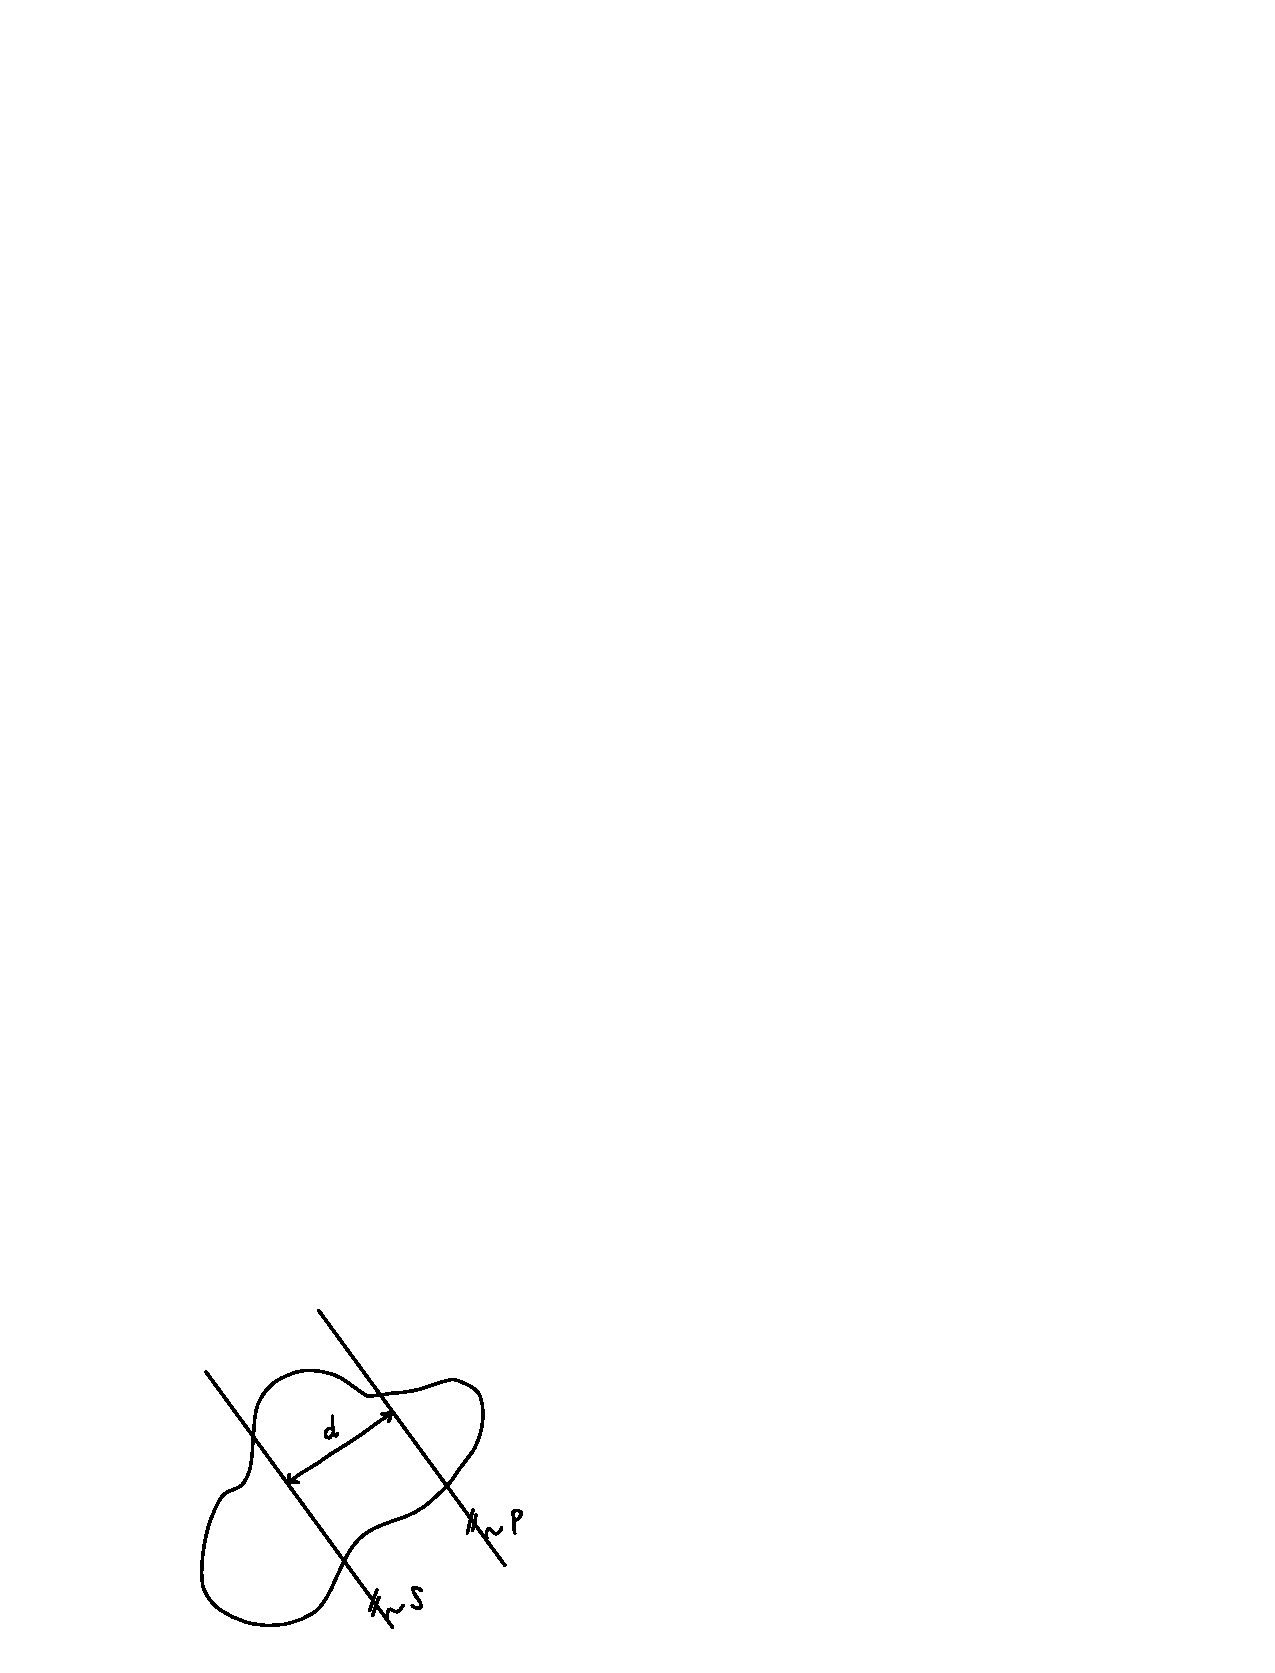
\includegraphics[width=\linewidth]{src/Mehrdimensionale-Funktionen_Integralrechnung/satz-von-steiner.pdf}
    \end{minipage}
    \hspace{0.05\linewidth}
    \begin{minipage}{0.4\linewidth}
        \begin{align*}
            I_p &=\,\, I_s + d^2 \cdot m\\
            m \vcentcolon&= Masse\\
            d \vcentcolon&= Abstand\\
        \end{align*}
    \end{minipage}
    %     % !TeX root = ../../ZF_bmicha_Ana.tex
\subsection{Leibnitz Theorem}
\vspace{-0.5em}
$$
    \frac{d}{dx} \left( \int_{a(x)}^{b(x)} f(x,t) dt \right) =
$$
$$
    \int_{a(x)}^{b(x)}  f_x(x,t) dt + f(x,b(x)) \, \frac{db(x)}{dx}  - f(x,a(x)) \, \frac{da(x)}{dx}
$$
\vspace{0.9em}

    %     % !TeX root = ../../ZF_bmicha_Ana.tex
\subsection{Oberflächenintegrale}
    Spezialfall eines Flächenintegrals.\\    
    Flächeninhalt einer parametr. Oberfläche berechnen:
    \mathbox{
        \iint_{\mathcal{O}} d\mathcal{O} = \iint_{\mathcal{O}} \abs*{\vec{r}_u \times \vec{r}_v} du dv
    }
    \textbf{Parametrisierung der Oberfläche:}
    $$
        \vec{r} = \begin{pmatrix}
            x(u,v)\\
            y(u,v)\\
            z(u,v)
        \end{pmatrix}
    $$
    \begin{description}
        \item[Oberflächenelement:] $d\mathcal{O} = \abs*{\vec{r}_u \times \vec{r}_v} du dv$
        \item[Normalenvektor:]  $\vec{n} = \vec{r}_u \times \vec{r}_v$
        \item[Normaleneinheitsvektor:]  $\vec{n}_o = \frac{\vec{r}_u \times \vec{r}_v}{\abs*{\vec{r}_u \times \vec{r}_v}}$
    \end{description}
    {\small Oberflächenelement entspricht Jacobi-Determinante.}
    % \cbreak
    %     % !TeX root = ../../ZF_bmicha_Ana.tex
\subsection{Flächenparametrisierungen}
Gängige Tricks falls die Fläche gegeben ist als:
    \begin{enumerate}
        \item $z = f(x,y)$
            $$
                \vec{r}(x,y) = \begin{pmatrix}
                    x\\y\\f(x,y)
                \end{pmatrix}
            $$
        \item $z = f(r,\varphi)$
            $$
                \vec{r}(r,\varphi) = \begin{pmatrix}
                    r\cos(\varphi)\\r\sin(\varphi)\\f(r,\varphi)
                \end{pmatrix}
            $$
        \item Rotationssymmetrische Fläche
            $$
                \vec{r}(t,\varphi) = \begin{bmatrix}
                    \mathrm{Rotations-}\\\mathrm{matrix}\\(\varphi)
                \end{bmatrix}
                \cdot
                \begin{pmatrix}
                    \mathrm{Param.}\\
                    \mathrm{Kurve}\\
                    \mathrm{(t)}
                \end{pmatrix}.
            $$
    \end{enumerate}
    \subsubsection{Rotationsmatrizen}
        \vspace{-1em}
        $$
        s_\varphi \vcentcolon= \sin(\varphi) \qquad c_\varphi \vcentcolon= \cos(\varphi)
        $$
        $$
        \begin{bmatrix}
            1 & 0 & 0\\
            0 & c_\varphi &-s_\varphi\\
            0 & s_\varphi & c_\varphi
        \end{bmatrix}_x
        \quad
        \begin{bmatrix}
            c_\varphi &0 & s_\varphi\\
            0 & 1 & 0\\
            -s_\varphi & 0 & c_\varphi
        \end{bmatrix}_y
        \quad\!
        \begin{bmatrix}
            c_\varphi &-s_\varphi& 0\\
            s_\varphi & c_\varphi& 0\\
            0 & 0 & 1
        \end{bmatrix}_z
        $$
    % \section{Vektoranalysis}
    %     % !TeX root = ../../ZF_bmicha_Ana.tex
Jedem Punkt im Raum $(x,y,z)$ wird ein Vektor zugeordnet.
% Bsp.: Geschwindigkeitsfeld eines Flusses - ''In welche Richtung fliesst das Wasser mit welcher Geschwindigkeit?''
$$
    \vec{v}(x,y,z) = \begin{pmatrix}
        u(x,y,z)\\v(x,y,z)\\w(x,y,z)
    \end{pmatrix}
$$
    %     % !TeX root = ../../ZF_bmicha_Ana.tex
\subsection{Allgemein}
    \textbf{Divergenz} (Quellstärke)
        $$
            \mathrm{div}(\vec{v}) = \nabla \cdot \vec{v} = u_x + v_y + w_z
        $$
    \textbf{Rotation} (Wirbelstärke)
        $$
            \mathrm{rot}(\vec{v}) = \nabla \times \vec{v} = 
            \begin{pmatrix}
                w_y - v_z\\ u_z - w_x\\v_x - u_y
            \end{pmatrix}
        $$
    \subsubsection{Identitäten}
        \vspace{-1em}
        \begin{align*}
            \div(\rot(\vvec)) = 0 && \rot(\grad(f)) = 0
        \end{align*}
    %     \vspace{-0.25em}
    %     % !TeX root = ../../ZF_bmicha_Ana.tex
\subsection{Fluss \hfill $\Phi$}
    \vspace{-1em}
    \begin{align*}
        \Phi &= \iint_A \vvec \cdot \novec \ dA &\textrm{Allgemein}\\
        \Phi &= \iint_A \vvec(\rvec(u,v)) \cdot (\rvec_u \times \rvec_v) \ du dv &\textrm{Parametr.}\\
        \Phi &= \iiint_V \div(\vvec) \ dV &\textbf{Satz\ v. Gauss}
    \end{align*}

    \subsubsection{Satz von Gauss}
        Falls $\vvec$ in ganz $B$ \textbf{definiert} und einmal \textbf{stetig differenzierbar} (\textit{regulär}) ist, gilt
        $$
            \iint_{\partial B} \vvec \cdot \novec \ dO = \iiint_B \div(\vvec) \ dV,
        $$
        wobei $\partial B$ die geschlossene Oberfläche des Volumens $B$ bezeichnet.
        Der Normaleneinheitsvektor $\novec$ auf $\partial B$ zeigt von innen nach aussen.
    %     % !TeX root = ../../ZF_bmicha_Ana.tex
\subsection{Arbeit \texorpdfstring{\hfill $W$}{W}}
    \vspace{-1em}
    \begin{align*}
        W &= \int_C \vvec \ d \vec{r} &\textrm{Allgemein}\\
        W &= \int_C \vvec(\rvec(t)) \cdot \dot{\rvec}(t) \ dt &\textrm{Parametr.}\\
        W &= \iint_{A} \rot(\vvec) \cdot \novec \ dA & \textrm{Satz von Stokes}\\[0.125em]
        W &= f\left(P_{\textrm{Ende}}\right) - f\left(P_{\textrm{Anfang}}\right) &\textrm{Potentialfeld}
    \end{align*}

    \subsubsection{Arbeit Berechnen}
        \vspace{0.5em}
        \resizebox*{0.99\linewidth}{!}{
            \tikzset{every picture/.style={line width=0.75pt}} %set default line width to 0.75pt        
            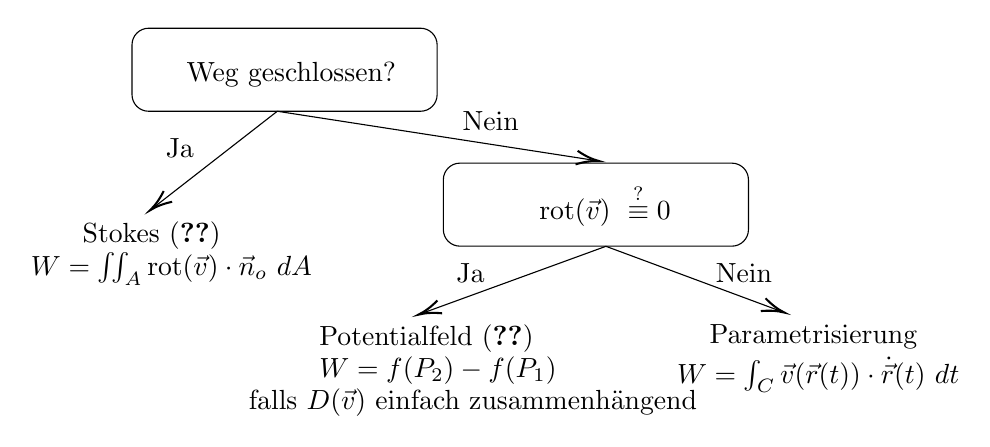
\begin{tikzpicture}[x=0.75pt,y=0.75pt,yscale=-1,xscale=1]
                \draw   (235,71) .. controls (235,66.58) and (238.58,63) .. (243,63) -- (374,63) .. controls (378.42,63) and (382,66.58) .. (382,71) -- (382,95) .. controls (382,99.42) and (378.42,103) .. (374,103) -- (243,103) .. controls (238.58,103) and (235,99.42) .. (235,95) -- cycle ;
                \draw   (385,136) .. controls (385,131.58) and (388.58,128) .. (393,128) -- (524,128) .. controls (528.42,128) and (532,131.58) .. (532,136) -- (532,160) .. controls (532,164.42) and (528.42,168) .. (524,168) -- (393,168) .. controls (388.58,168) and (385,164.42) .. (385,160) -- cycle ;
                \draw    (305,103) -- (245.25,149.5) ;
                \draw [shift={(243.67,150.73)}, rotate = 322.11] [color={rgb, 255:red, 0; green, 0; blue, 0 }  ][line width=0.75]    (10.93,-3.29) .. controls (6.95,-1.4) and (3.31,-0.3) .. (0,0) .. controls (3.31,0.3) and (6.95,1.4) .. (10.93,3.29)   ;
                \draw    (305,103) -- (458.02,126.69) ;
                \draw [shift={(460,127)}, rotate = 188.8] [color={rgb, 255:red, 0; green, 0; blue, 0 }  ][line width=0.75]    (10.93,-3.29) .. controls (6.95,-1.4) and (3.31,-0.3) .. (0,0) .. controls (3.31,0.3) and (6.95,1.4) .. (10.93,3.29)   ;
                \draw    (463.33,168.07) -- (374.88,200.31) ;
                \draw [shift={(373,201)}, rotate = 339.97] [color={rgb, 255:red, 0; green, 0; blue, 0 }  ][line width=0.75]    (10.93,-3.29) .. controls (6.95,-1.4) and (3.31,-0.3) .. (0,0) .. controls (3.31,0.3) and (6.95,1.4) .. (10.93,3.29)   ;
                \draw    (463.33,168.07) -- (547.46,199.3) ;
                \draw [shift={(549.33,200)}, rotate = 200.37] [color={rgb, 255:red, 0; green, 0; blue, 0 }  ][line width=0.75]    (10.93,-3.29) .. controls (6.95,-1.4) and (3.31,-0.3) .. (0,0) .. controls (3.31,0.3) and (6.95,1.4) .. (10.93,3.29)   ;

                % Text Node
                \draw (260,78) node [anchor=north west][inner sep=0.75pt]   [align=left] {Weg geschlossen?};
                % Text Node
                \draw (430,137) node [anchor=north west][inner sep=0.75pt]    {$\text{rot}(\vec{v}) \ \overset{?}{\equiv} 0$};
                % Text Node
                \draw (210,155) node [anchor=north west][inner sep=0.75pt]   [align=left] {Stokes (\ref{sec:SatzVonStokes})};
                % Text Node
                \draw (324,204.5) node [anchor=north west][inner sep=0.75pt]   [align=left] {Potentialfeld (\ref{sec:Potentialfeld})};
                % Text Node
                \draw (512,204.5) node [anchor=north west][inner sep=0.75pt]   [align=left] {Parametrisierung};
                % Text Node
                \draw (250,114.9) node [anchor=north west][inner sep=0.75pt]   [align=left] {Ja};
                % Text Node
                \draw (390,175) node [anchor=north west][inner sep=0.75pt]   [align=left] {Ja};
                % Text Node
                \draw (393,102) node [anchor=north west][inner sep=0.75pt]   [align=left] {Nein};
                % Text Node
                \draw (515,175) node [anchor=north west][inner sep=0.75pt]   [align=left] {Nein};
                % Text Node
                \draw (185,170) node [anchor=north west][inner sep=0.75pt]    {$W = \iint_{A} \rot(\vvec) \cdot \novec \ dA$};
                % Text Node
                \draw (324,220) node [anchor=north west][inner sep=0.75pt]    {$W = f(P_2) - f(P_1)$};
                \draw (290,235.5) node [anchor=north west][inner sep=0.75pt]    {falls $D(\vvec)$ einfach zusammenhängend};
                % Text Node
                \draw (496.33,220) node [anchor=north west][inner sep=0.75pt]    {$W = \int_C \vvec(\rvec(t)) \cdot \dot{\rvec}(t) \ dt$};
            \end{tikzpicture}
        }

    \subsubsection{Satz von Stokes} \label{sec:SatzVonStokes}
        Falls $\vvec$ auf ganz $A$ \textbf{definiert} und \textbf{stetig differenzierbar} (\textit{regulär}) ist, gilt
        $$
            \int_{\partial A} \vvec \ d \rvec = \iint_{A} \rot(\vvec) \cdot \novec \ dA,
        $$
        wobei $\partial A$ den geschlossenen Rand der Fläche $A$ bezeichnet.
        Der Normaleneinheitsvektor $\novec$ auf $A$ beschreibt mit der \textit{Rechte-Hand-Regel} den Umlaufsinn von $\partial A$.

    \subsubsection{Potentialfeld \texorpdfstring{$\vvec$}{v} zum Potential \texorpdfstring{$f$}{f}} \label{sec:Potentialfeld}
        Falls der Definitionsbereich $D(f)$ eines \textbf{wirbel\-freien} ($\rot(\vvec) \equiv 0$) Vektorfeldes \textbf{einfach zusammenhängend} (EZH) ist, nennen wir es \textit{konservativ}:
        \mathbox{
           D(f) \textrm{ EZH }\  \textit{und }\ \rot(\vvec) \equiv \vec{0} \quad \Rightarrow \quad \vvec = \grad(f).
        }
        $$ 
        \vvec = 
        \begin{pmatrix}
            u\\v\\w
        \end{pmatrix}
        =
        \begin{pmatrix}
            f_x\\f_y\\f_z
        \end{pmatrix}
        = \grad(f)
        $$ 

        $$
            f(x,y,z) = \int u \ dx = \int v \ dy = \int w \ dz
        $$
        Die Arbeit zwischen zwei Punkten entspricht der Potentialdifferenz.
        % \mathbox{
        %         $\vvec$ Potentialfeld &$\Longrightarrow$ $\rot(\vvec)=\vec{0}$
        % }
        \begin{empheq}[box=\fbox]{align*}
            \vvec \textrm{ Potentialfeld } &\Longrightarrow \rot(\vvec)=\vec{0}\\
            \vvec \textrm{ Potentialfeld } &\Longleftarrow \rot(\vvec)=\vec{0} \textrm{ \& } D(\vvec) = \textrm{ EZH}
        \end{empheq}
    
    
    %     % !TeX root = ../../ZF_bmicha_Ana.tex
\subsection{DGLs \& Vektorfelder}
    \vspace{0.5em}
    \mathbox[$\qquad \vvec = \begin{pmatrix} v_1\\v_2 \end{pmatrix}$]{
        y' = \frac{v_2}{v_1}
    }
    \subsubsection{Feldlinien \texorpdfstring{$y(x)$}{y(x)} \texorpdfstring{$\to$}{->} Vektorfeld \texorpdfstring{$\vvec$}{v}}
        \begin{enumerate}
            \item Feldliniengleichung nach $x$ ableiten $\to$ $y'(x)$
            \item Scharparameter eliminieren
            \item $\displaystyle y' = \frac{v_2}{v_1}$ $\to$ $\vvec = \begin{pmatrix} v_1\\v_2 \end{pmatrix}$
        \end{enumerate}
    \subsubsection{Vektorfeld \texorpdfstring{$\vvec$}{v} \texorpdfstring{$\to$}{->} Feldlinien \texorpdfstring{$y(x)$}{y(x)}}
        \vspace{0.5em}
        \begin{enumerate}
            \item $\displaystyle y' = \frac{v_2}{v_1}$
            \item DGL lösen
        \end{enumerate}
    % \section{Differentialgleichungen (DGL)}
    %     % !TeX root = ../../ZF_bmicha_Ana.tex
\subsection{Eigenschaften}
    \subsubsection{Existenz- \& Eindeutigkeitssatz}
        Sei $y' = f(x,y)$ in $D(f)$ \textbf{stetig} und \textbf{stetig partiell nach $\boldsymbol{y}$ differenzierbar}.
        \begin{itemize}
            \item[$\Rightarrow$] Für jeden Punkt $(x_o,y_o) \in D(f)$ gibt es \textit{genau eine} Lösung. 
            \item[$\Rightarrow$] Graphen von versch. Anfangswertproblemen (AWP) sind identisch oder disjunkt (kein gem. Pkt.).
        \end{itemize}
    \subsubsection{Linear}
        Eine DGL heisst \textit{linear}, falls alle $y$-Terme ($y, y', y'', \dots$) nur linear vorkommen.
        ($\to$ Kein: $sin(y')$, $y\cdot y'$, $e^y$, \dots)

% \textbf{Nützliche Integrale}
%     \begin{align*}
%         \int \frac{a}{ax + b} \ dx &= \ln(ax + b) + C, \quad C \in \mathbb{R}\\
%         \int \frac{\frac{1}{a}}{1 + \left(\frac{x}{a}\right)^2} \ dx &= \arctan\left(\frac{x}{a}\right) + C, \quad C \in \mathbb{R}
%     \end{align*}
% \textbf{Ordnung:}\\
%     Die Ordnung einer DGL entspricht dem Grad der höchsten Ableitung.
    %     % !TeX root = ../../ZF_bmicha_Ana.tex
\subsubsection{Separierbar} \label{sec:separierbareDGL}
    Separierbare DGLs können auf folgende Form gebracht werden:
    \mathbox{
        h(y(x)) \cdot y'(x) = g(x).
    }
    \begin{align*}
        h(y(x)) \cdot \frac{dy}{dx} &= g(x)\\
        \int h(y(x)) \cdot dy &= \int g(x) \cdot dx
    \end{align*}
    %     % !TeX root = ../../ZF_bmicha_Ana.tex
\subsubsubsection{Substitutionen}
    \begin{align*}
        u(x) &= \frac{y}{x}\\
        u(x) &= ax + by(x) + c\\
        u(x) &= y'(x)    
    \end{align*}
    Um $y'$ zu ersetzen, Substitution nach $y$ umformen und nach $x$ ableiten.
    %     % !TeX root = ../../ZF_bmicha_Ana.tex
\subsection{Orthogonaltrajektorien}
    \vspace{0.5em}
    \mathbox{
        y' = - \frac{1}{y_{OT}'}
    }
    \begin{enumerate}
        \item Kurvenschar $y(x)$ ableiten $\to y'(x)$
        \item Scharparameter eliminieren
        \item Obige Relation einsetzen und $y \to y_{OT}$
        \item DGL für $y_{OT}$ lösen
    \end{enumerate}
    %     % !TeX root = ../../ZF_bmicha_Ana.tex
\subsection{Enveloppe / Umhüllende} \label{sec:Enveloppe}
    \begin{empheq}[box=\fbox]{align*}
        F(x,y,C) &= 0\\
        \frac{\partial}{\partial C}F(x,y,C) &= 0
    \end{empheq}
    \begin{enumerate}
        \item Darstellung der Kurvenschar mit Scharparameter C finden: $F(x,y,C) = 0$
        \item Ausdruck für Scharparam. mit obigen Gleichungen bestimmen.
        \item Gefundenen Ausdruck $\widetilde{C}$ für Scharparam. in $F(x,y,C) = 0$ einsetzen $\to$ Enveloppengleichung
    \end{enumerate}
    %     % !TeX root = ../../ZF_bmicha_Ana.tex
\subsection{Lineare DGL 1. Ordnung}
    \vspace{0.5em}
    \mathbox%[$\quad q(x) \vcentcolon=$ Störfunktion]
    {
        y' + p(x) \cdot y = q(x)
    }
    $\triangleright$ $q(x) \vcentcolon=$ Störfunktion
    
    \subsubsection{Homogen \texorpdfstring{$\hfill q(x) \equiv 0$}{q(x) = 0}}
        \vspace{0.5em}
        \mathbox{
            y' + p(x) \cdot y = 0
        }
        $\triangleright$ Immer separierbar. (\ref{sec:separierbareDGL})
    \subsubsection{Inhomogen \texorpdfstring{$\hfill q(x) \neq 0$}{q(x) =/= 0}}\label{sec:1.Ord-homogen}
        \vspace{0.5em}
        \mathbox{
            y' + p(x) \cdot y = q(x)
        }
        \begin{enumerate}
            \item $q(x) = 0$ setzen, homogene Lösung $y_h$ finden
            % $y_h' + p(x) \cdot y_h = 0$
            \item Partikuläre Lösung $y_p$ finden:
            \begin{itemize}
                \item Ansatz von Tabelle %(\ref{sec:linh-1orderTabelle})
                \item Lagrange-Methode %(\ref{sec:linh-1orderLagrange})
            \end{itemize}
        \end{enumerate}

        \subsubsubsection{Ansatz}
            \begin{enumerate}
                \item Ansatz für $y_p$ in inhomogene DGL einsetzen
                \item Koeffizientenvergleich
                \item $y = y_h + y_p$
            \end{enumerate}
            \begin{center}
                \renewcommand{\arraystretch}{1.25}
                \begin{tabular}{ll}
                    \hline
                    Störfunktion $q(x)$                                                                                                                       & Ansatz für $y_p(x)$                          \\ \hline\hline
                    Konstante                                                                                                                                 & $y_p = A$                                    \\
                    lineare Fkt.                                                                                                                              & $y_p = Ax + B$                               \\
                    Polynom Grad $n$                                                                                                                          & $y_p = Ax^n + Bx^{n-1} + \cdots$             \\
                    \begin{tabular}[c]{@{}l@{}}$A \sin(\omega x), A \cos( \omega x),$ \phantom{dirtl} \\ $A \sin(\omega x) + B \cos( \omega x)$\end{tabular} & $y_p = C \sin(\omega x) + D \cos( \omega x)$  \\
                    $A e^{{\color{blue}b}x}$                                                                                                                  & $y_p = B e^{{\color{blue}b}x}$               \\\hline
                \end{tabular}
                
                \vspace{0.5em}
                \textit{Ansatz funktioniert nicht $\to$ mit $x$ multiplizieren.}
            \end{center}

        \subsubsubsection{Lagrange-Methode}
            \begin{enumerate}
                \item Lagrange-Ansatz $y_p$:\ $y_h = C \cdots \to y_p = C(x) \cdots$
                \item Ansatz in inhomogene DGL einsetzen
                \item Nach $C'(x)$ auflösen und integrieren
                \item $C(x)$ in $y_p$ einsetzen
                \item $y = y_p$
            \end{enumerate}
    %     % !TeX root = ../../ZF_bmicha_Ana.tex
\subsection{DGL Spezialfälle}
    \subsubsection{Clairaut'sche DGL}
        Entspricht Geraden mit Steigung $y'$ und Achsenabschnitten $g(y')$.
        \mathbox{
            y = y' \cdot x + g(y')
        }
        \begin{itemize}
            \item \textbf{Allgemeine Lösung:}
            $$
                y = C\cdot x + g(C)
            $$
            \item \textbf{Singuläre Lösung:}\\
                Enveloppe der allg. Lsg. bestimmen. (\ref{sec:Enveloppe})
        \end{itemize}

    \subsubsection{Exakte DGL}
        \vspace{0.5em}
        \mathbox{
            f_x + f_y \cdot y' = 0
        }
        \begin{itemize}
            \item Bedingung: $f_{xy} = f_{yx}$
            \item Allgemeine Lösung: $f(x,y) = C$
        \end{itemize}
    %     % !TeX root = ../../ZF_bmicha_Ana.tex
\subsection{Lineare DGL n. Ordnung - konst. Koeff.}
    \subsubsection{Homogen}\label{sec:konst-koeff-homogen}
        \vspace{0.5em}
        \mathbox{
            a_n y^{(n)} + \cdots + a_2 y'' + a_1 y' + a_0 y = 0
        }
        \begin{enumerate}
            \item Ansatz \fbox{$y=e^{\lambda x}$} einsetzen $\to$ \textbf{char. Polynom}
            \item Nullstellen $\lambda_i$ des char. Polynom bestimmen
            \begin{itemize}
                \item $\lambda_1 \neq \lambda_2 \neq \cdots$, reell
                    $$
                        y = C_1 e^{\lambda_1 x} + C_2 e^{\lambda_2 x} + C_3 e^{\lambda_3 x}+ \cdots
                    $$
                \item $\lambda_1 = \lambda_2 = \cdots$, reell
                    $$
                        y = C_1 e^{\lambda_1 x} + C_2 {\color{magenta} x} e^{\lambda_2 x} + C_3 {\color{magenta} x^2} e^{\lambda_3 x} + \cdots
                    $$
                \item $\lambda_{1,2} = \lambda_{3,4} = \cdots = {\color{red}a} \pm i {\color{blue}b}$
                    \begin{align*}
                        y =\phantom{x} &e^{{\color{red}a}x} (C_1 \cos({\color{blue}b}x) + C_2 \sin({\color{blue}b}x)) +\\
                            {\color{magenta} x}&e^{{\color{red}a}x} (C_3 \cos({\color{blue}b}x) + C_4 \sin({\color{blue}b}x))+\\
                            {\color{magenta} x^2}&e^{{\color{red}a}x} (C_5 \cos({\color{blue}b}x) + C_6 \sin({\color{blue}b}x))+ \cdots
                    \end{align*}
            \end{itemize}
        \end{enumerate}
    \subsubsection{Inhomogen}
        \vspace{0.5em}
        \mathbox{
            a_n y^{(n)} + \cdots + a_2 y'' + a_1 y' + a_0 y = q(x)
        }
        \begin{enumerate}
            \item Homogene Lösung $y_h$ bestimmen (\ref{sec:konst-koeff-homogen})
            \item Partikuläre Lösung $y_p$
            \begin{itemize}
                \item Ansatz wie gewohnt (\ref{sec:1.Ord-homogen})\\
                      Ansatz klappt nicht $\to$ mit $x$ multiplizieren
                \item Lagrange-Methode (\ref{sec:Lagrange-2-Ordnung})
            \end{itemize}
        \end{enumerate}
    %     \cbreak
    %     % !TeX root = ../../ZF_bmicha_Ana.tex
\subsection{Lagrange-Methode 2. Ordnung}\label{sec:Lagrange-2-Ordnung}
    \begin{enumerate}
        \item DGL auf folgende Form bringen:
            $$
                y'' + p_0(x) y' + p_1(x)y = q(x)
            $$
        \item Homogene Lösung
            $$
                y_h =\, C_1\,y_1(x) + C_2\,y_2(x)
            $$
        \item $C_1(x), C_2(x)$ bestimmen
            \begin{align*}
                C_1(x) &= - \int \frac{q(x) y_2(x)}{W(x)} dx\\[0.25em]
                C_2(x) &= \phantom{-}\int \frac{q(x) y_1(x)}{W(x)} dx
            \end{align*}
            \vspace{0.5em}
            $$
                W(x) = y_1y_2' - y_1'y_2 \qquad q(x) = \textrm{Störterm}
            $$
        \item Allgemeine Lösung
            \mathbox{
                y =\, C_1(x)\,y_1(x) + C_2(x)\,y_2(x)
            }
        
    \end{enumerate}
    %     % !TeX root = ../../ZF_bmicha_Ana.tex
\subsection{Euler DGL}
    \subsubsection{Homogen}\label{sec:Euler-homogen}
        \vspace{0.5em}
        \mathbox{
            a_n x^n y^{(n)} + \cdots + a_2 x^2 y'' + a_1 x y' + a_0 y = 0
        }
        \begin{enumerate}
            \item Ansatz \fbox{$y=x^\alpha$} einsetzen $\to$ \textbf{Indexpolynom}
            \item Nullstellen $\alpha_i$ des Indexpolynom bestimmen
            \begin{itemize}
                \item $\alpha_1 \neq \alpha_2 \neq \cdots$, reell
                    $$
                        y = C_1 x^{\alpha_1} + C_2 x^{\alpha_2} + C_3 x^{\alpha_3}+ \cdots
                    $$
                \item $\alpha_1 = \alpha_2 = \cdots$, reell
                    $$
                        y = C_1 x^{\alpha_1} + C_2 {\color{magenta} \ln(x)} x^{\alpha_2} + C_3 {\color{magenta} \ln(x)^2} x^{\alpha_3} + \cdots
                    $$
                \item $\alpha_{1,2} = \alpha_{3,4} = \cdots = {\color{red}a} \pm i {\color{blue}b}$
                    \begin{align*}
                        y =\phantom{\ln} &x^{{\color{red}a}} (C_1 \cos({\color{blue}b} \ln(x)) + C_2 \sin({\color{blue}b} \ln(x))) +\\
                            {\color{magenta} \ln(x)}&x^{{\color{red}a}} (C_3 \cos({\color{blue}b} \ln(x)) + C_4 \sin({\color{blue}b} \ln(x)))+\\
                            {\color{magenta} \ln(x)^2}&x^{{\color{red}a}} (C_5 \cos({\color{blue}b} \ln(x)) + C_6 \sin({\color{blue}b} \ln(x)))+ \cdots
                    \end{align*}
            \end{itemize}
        \end{enumerate}
    \subsubsection{Inhomogen}
        \vspace{0.5em}
        \mathbox{
            a_n x^n y^{(n)} + \cdots + a_2 x^2 y'' + a_1 x y' + a_0 y = q(x)
        }
        \begin{enumerate}
            \item Homogene Lösung $y_h$ bestimmen (\ref{sec:Euler-homogen})
            \item Partikuläre Lösung $y_p$
            \begin{itemize}
                \item Ansatz (\ref{sec:1.Ord-homogen})\\
                      Ansatz klappt nicht $\to$ mit $\ln(x)$ multiplizieren
                \item Lagrange-Methode (\ref{sec:Lagrange-2-Ordnung})
            \end{itemize}
        \end{enumerate}
    %     \cbreak
    %     % !TeX root = ../../ZF_bmicha_Ana.tex
\subsection{DGL Systeme}
    \vspace{0.5em}
    \begin{minipage}{0.5\linewidth}
        \centering
        \textbf{Allgemein:}
        \begin{align*}
            y_1'(x) &= f_1(x,y_1,y_2)\\
            y_2'(x) &= f_2(x,y_1,y_2)
        \end{align*}
    \end{minipage}
    \begin{minipage}{0.48\linewidth}
        \centering
        \textbf{Autonom:}
        \begin{align*}
            y_1'(x) &= f_1(y_1,y_2)\\
            y_2'(x) &= f_2(y_1,y_2)
        \end{align*}
    \end{minipage}
    \vspace{0.5em}
    \begin{itemize}
        \item Ein DGL System heisst \textbf{autonom}, falls die zu den gesuchten Funktionen ($y_1, y_2$) gehörige Variable ($x$) nicht explizit vorkommt.
    \end{itemize}

    \subsubsection{Existenz- \& Eindeutigkeitssatz}
        Die Funktionen $f_1,f_2$ seien \textbf{stetig in $\boldsymbol{x}$} und \textbf{stetig partiell nach $\boldsymbol{y_1,y_2}$ differenzierbar}.
        \begin{itemize}
            \item[$\Rightarrow$] Zu vorgegebenem $x_o, y_{1,o}, y_{2,o}$ gibt es \textit{genau ein Paar} $f_1,f_2$, welches das System löst und das AWP $y_1(x_o) = y_{1,o}$ und $y_2(x_o) = y_{2,o}$ erfüllt.
        \end{itemize}
    \subsubsection{Lineare Autonome DGL Systeme mit konstanten Koeffizienten}
        \vspace{-0.5em}
        $$
            \dot{x} = A \cdot x + b
        $$
        \vspace{0em}
        $$
            \underbrace{\begin{pmatrix}
                \dot{x}_1\\ \dot{x}_2
            \end{pmatrix}}_{\dot{x}}
            =
            \underbrace{\begin{bmatrix}
                a_{11} & a_{12}\\ a_{21} & a_{22}
            \end{bmatrix}}_{A}
            \cdot
            \underbrace{\begin{pmatrix}
                x_1\\ x_2
            \end{pmatrix}}_{x}
            +
            \underbrace{\begin{pmatrix}
                b_1\\ b_2
            \end{pmatrix}}_{b}
        $$
    \begin{itemize}
        \item \textbf{Eliminationsverfahren}
            \begin{enumerate}
                \item Nach einer gesuchten Funktion auflösen, ableiten und einsetzen
                \item DGL 2. Ordnung lösen
                \item Zweite gesuchte Funktion bestimmen
            \end{enumerate}
        \item \textbf{Linalg-Methode}
            \begin{enumerate}
                \item Eigenwerte $\lambda_i$ (EW) bestimmen
                    $$
                        0 \overset{!}{=} \det (A - \lambda \mathbb{I})
                    $$
                \item Eigenvektoren $\vvec_i$ zu EW $\lambda_i$ bestimmen
                    $$
                        (A - \lambda_i \mathbb{I}) \cdot \vvec_i \overset{!}{=} 0
                    $$
                \item Lösung Konstruieren:
                \begin{itemize}
                    \item $\lambda_{1,2}$ reell
                        \mathbox{
                            \begin{pmatrix}
                                x_1\\x_2
                            \end{pmatrix}
                            = 
                            C_1 \cdot \vvec_1 \cdot e^{\lambda_1 t}
                            +
                            C_2 \cdot \vvec_2 \cdot e^{\lambda_2 t}
                        }
                    \item $\lambda_{1,2} = a \pm ib$ 
                        $$
                            \lambda_{1} = a + ib \quad \to \quad \vvec_1 =
                            \begin{pmatrix}
                                c\\id
                            \end{pmatrix}
                        $$
                        $$
                            w = 
                            \vvec_1 \cdot e^{\lambda_1 t}
                            =
                            \begin{pmatrix}
                                c\\id
                            \end{pmatrix}
                            e^{(a+ib)t}
                        $$
                        \mathbox{
                            \begin{pmatrix}
                                x_1\\x_2
                            \end{pmatrix}
                            = 
                            C_1 \cdot \textrm{Re}(\wvec)
                            +
                            C_2 \cdot \textrm{Im}(\wvec)
                        }

                \end{itemize}

            \end{enumerate}
            

    \end{itemize}
    
    \subsubsection{Gleichgewichtspunkte (GGWP)}
        $$
            \begin{pmatrix}
                \dot{x}\\ \dot{y}
            \end{pmatrix}
            =
            \begin{pmatrix}
                f_1(x,y)\\ f_2(x,y)
            \end{pmatrix}
            \overset{!}{=} 
            \begin{pmatrix}
                0\\0
            \end{pmatrix}
        $$
    \subsubsection{Stabilitätsverhalten}
        \vspace{-1em}
        \begin{align*}
            \dot{x} = f_1(x,y)\\
            \dot{y} = f_2(x,y)
        \end{align*}
        \vspace{-0.75em}
        \begin{enumerate}
            \item Falls nötig um GGWP $(x_o,y_o)$ linearisieren:
                  $$
                    \begin{pmatrix}
                        \dot{\xi}\\[0.5em] \dot{\eta}
                    \end{pmatrix}
                    =
                    \underbrace{\begin{bmatrix}
                        \frac{\partial f_1}{\partial x}(x_o, y_o) & \frac{\partial f_1}{\partial y}(x_o, y_o)\\[0.5em]
                        \frac{\partial f_2}{\partial x}(x_o, y_o) & \frac{\partial f_2}{\partial y}(x_o, y_o)
                    \end{bmatrix}}_{A}
                    \cdot 
                    \begin{pmatrix}
                        \xi\\[0.5em] \eta
                    \end{pmatrix}
                  $$
            \item Eigenwerte $\lambda_i$ von $A$ bestimmen
            \begin{itemize}
                \item Re$(\lambda_i) < 0, \ \forall i \quad \to $ \textit{asymptotisch stabil}
                \item Re$(\lambda_i) \leq 0, \ \forall i \quad \to $ \textit{stabil}
                \item Re$(\lambda_i) > 0, \ \exists i \quad \to $ \textit{instabil}
            \end{itemize}
        \end{enumerate}
    \subsubsection{Phasenportrait}
        Die Feldlinien des Vektorfeldes $\vvec$ beschreiben die Lösungskurven des \textit{autonomen} DGL Systems.
        $$
            \vvec =
            \begin{pmatrix}
                \dot{x}\\ \dot{y}
            \end{pmatrix}
            =
            \begin{pmatrix}
                f_1(x,y)\\f_2(x,y)
            \end{pmatrix}
        $$
        \vspace{0.5em}
        $$
            y_{pp}' = \frac{v_2}{v_1}
        $$  
    %\vfill \null \columnbreak
    \section{Appendix}
    % !TeX root = ../../ZF_bmicha_Ana.tex
\subsection{Nullstellen Reeller Polynome mit Grad}
    \vspace{-1em}
    $$
        p(x) = a_0 + a_1 x + a_2 x^2 + \dots + a_n x^n, \qquad a_i \in \mathbb{R}
    $$
    \begin{itemize}
        \item Hat genau $n$ Nullstellen (komplex und reell)
        \item Komplexe Nullstellen kommen immer im komplex-konjugierten Paar vor.
    \end{itemize}
    % !TeX root = ../../ZF_bmicha_Ana.tex
\subsection{Cosinus und Sinus - Integrale}
    Für $a,b \in \mathbb{Z}$ und $n \geq 2$, gelten:
    \begin{align*}
        \int_{a \cdot \frac{\pi}{2}}^{b \cdot \frac{\pi}{2}} \sin^n(x) \ dx 
            &= \frac{n-1}{n} \int_{a \cdot \frac{\pi}{2}}^{b \cdot \frac{\pi}{2}} \sin^{n-2}(x) \ dx\\[0.5em]
        \int_{a \cdot \frac{\pi}{2}}^{b \cdot \frac{\pi}{2}} \cos^n(x) \ dx 
            &= \frac{n-1}{n} \int_{a \cdot \frac{\pi}{2}}^{b \cdot \frac{\pi}{2}} \cos^{n-2}(x) \ dx
    \end{align*}
    Diese Regel kann mehrfach angewandt werden.
    % !TeX root = ../../ZF_bmicha_Ana.tex
\subsection{Ableitung Un-/Gerader Funktionen}
\begin{itemize}
    \item $g(x)$ sei \textbf{gerade}
        $$
            g'(0)=g^{(3)}(0)=g^{(5)}(0)=...=0
        $$
    \item $f(x)$ sei \textbf{ungerade}
        $$
            f''(0)=f^{(4)}(0)=f^{(6)}(0)=...=0
        $$
\end{itemize}
    \subsection{Rechengesetze für Exponenten \& Logarithmen}
\vspace*{-1em}
    \begin{align*}
        B^a \cdot B^b =& \; B^{a + b}\\
        \frac{B^a}{B^b} =& \; B^{a - b}\\
        (B^a)^b =& \; B^{a \cdot b}\\
        \log_B (a \cdot b ) =& \; \log_B (a) + \log_B (b)\\
        \log_B \left( \frac{a}{b} \right) =& \; \log_B (a) - \log_B (b)\\
        \log_B (a^r) =& \; r \cdot \log_B (a)\\
        \textrm{Basiswechsel: } \log_a (x) =& \; \frac{\log_b(x)}{\log_b(a)}
    \end{align*}
    \subsection{Polarkoordinaten}
    Umrechnung im ersten Quadranten
    \begin{align*}
        \begin{rcases}
            r = \rho(\phi)\\
            x = \cos(\phi) \cdot r\\
            y = \sin(\phi) \cdot r
        \end{rcases} \phi \in \left[0, \frac{\pi}{2}\right]
    \end{align*}
    \subsection{Häufige Parametrisierungen}
    \subsubsection{Ellipse}
    \vspace{0.5em}
    \mathbox{
        \overrightarrow{r}(t) = \binom{a \cdot cos(t) + x_0}{b \cdot sin(t) + y_0}
    }
    \text{Sonderfall Kreis mit Radius } a = b
    \begin{center}
        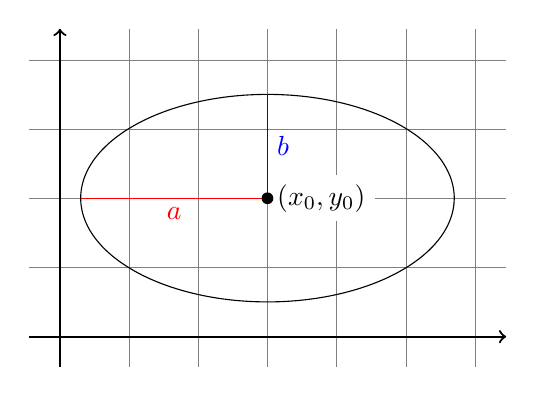
\begin{tikzpicture}[x=0.75pt,y=0.75pt,yscale=-1,xscale=1]
            %coordinatum system
            \foreach \i in {0, ..., 6} {
                \draw [very thin,gray] (\i * 33.33, -15) -- (\i * 33.33, 148);
            }
            \foreach \i in {0, ..., 4} {
                \draw [very thin,gray] (-15 ,\i * 33.33) -- (215 ,\i * 33.33);
            }
            \draw[thick, <-] (0, -15) -- (0, 148);
            \draw[thick, ->] (-15, 133.33) -- (215, 133.33);
            %
            %Ellipse
            \draw plot [smooth, samples = 100, domain = 0:500] ({90 * cos(\x) + 100}, {50 * sin(\x) + 66.6});
            %a
            \draw [red] (100, 66.66) -- (55, 66.66) node[anchor = north, red] {$a$} -- (10, 66.66);
            %b
            \draw [blue] (100, 66.66) -- (100, 41.66) node[anchor = west, blue] {$b$} -- (100, 16.66);
            %Midpoint
            \draw (100, 66.66) node[right, fill=white] {$(x_0, y_0)$} node[circle, fill, inner sep = 1.5pt]{};
        \end{tikzpicture}\\
    \end{center}
    
    \subsubsection{Zykloide}
    \vspace{0.5em}
    \mathbox{
        \overrightarrow{r}(t) = \binom{rt - a \sin(t)}{r - a \cos(t)}
    }
    \text{Sonderfall Gewöhnliche Zykloide } r = a\\
    \begin{center}
        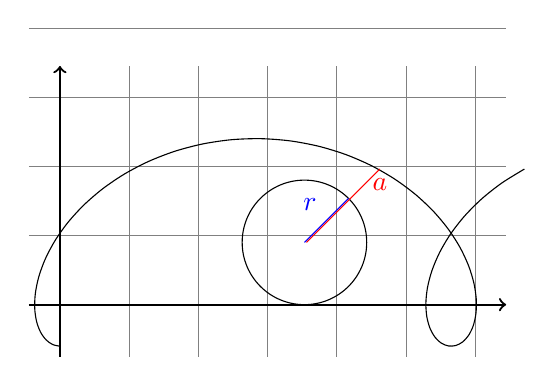
\begin{tikzpicture}[x=0.75pt,y=0.75pt,yscale=1,xscale=1]
            %coordinatum system
            \foreach \i in {0, ..., 6} {
                \draw [very thin,gray] (\i * 33.33, -25) -- (\i * 33.33, 115);
            }
            \foreach \i in {0, ..., 4} {
                \draw [very thin,gray] (-15 ,\i * 33.33) -- (215 ,\i * 33.33);
            }
            \draw[thick, ->] (0, -25) -- (0, 115);
            \draw[thick, ->] (-15, 0) -- (215, 0);
            %
            %Zykloide
            \draw plot [smooth, variable=\x, domain=0:2.75*pi, samples = 50] ({30 * \x - 50 * sin(\x*180/pi)},{30 - 50 * cos(\x*180/pi)});
            %circle
            \draw ({30 * (1.25 * pi)}, 30) circle (30);
            %a
            \draw [red] ({1 + 30 * (1.25 * pi)}, 30) -- ({1 + 30 * (1.25 * pi) - 50 * sin((1.25 * pi)*180/pi)}, {30 - 50 * cos((1.25 * pi)*180/pi)}) node[anchor = north, red] {$a$};
            %radius
            \draw [blue] ({30 * (1.25 * pi)}, 30) -- ({(30 * (1.25 * pi) + 30 * (1.25 * pi) + 30 * 1.414/2)/2}, {(30 + 30 + 30 * 1.414/2)/2}) node[anchor = south east, blue] {$r$} -- ({30 * (1.25 * pi) + 30 * 1.414/2}, {30 + 30 * 1.414/2});
            %
        \end{tikzpicture}\\
    \end{center}

    \vfill \null \columnbreak

    \subsubsection{Epizykloide}
    \vspace{0.5em}
    \mathbox{
        \overrightarrow{r}(t) = \binom{R cos(t) - a cos(\frac{R}{r} t)}{R sin(t) - a sin(\frac{R}{r} t)}
    }
    \text{Sonderfall Kardioide } R = 2r, r = a\\
    \begin{center}
        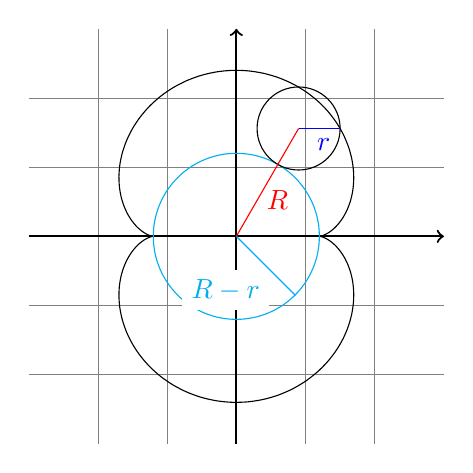
\begin{tikzpicture}[x=0.75pt,y=0.75pt,yscale=1,xscale=1]
            %coordinatum system
            \foreach \i in {-2, ..., 2} {
                \draw [very thin,gray] (\i * 33.33, -100) -- (\i * 33.33, 100);
            }
            \foreach \i in {-2, ..., 2} {
                \draw [very thin,gray] (-100 ,\i * 33.33) -- (100 ,\i * 33.33);
            }
            \draw[thick, ->] (0, -100) -- (0, 100);
            \draw[thick, ->] (-100, 0) -- (100, 0);
            %
            %Epizykloide
            \draw plot [smooth, variable=\x, domain=0:2*pi, samples = 100] ({60 * cos(\x*180/pi) - 20 * cos(60/20 * \x*180/pi)},{60 * sin(\x*180/pi) - 20 * sin(60/20 * \x*180/pi)});
            %big circle
            \draw [cyan] (0, 0) circle (40);
            \draw [cyan] (0, 0) -- (1.424/4 * 45, -1.424/4 * 45) node[anchor = north east, cyan, fill=white] {$R-r$} -- (1.424/2 * 40, -1.424/2 * 40);
            %small circle (t = pi/3)
            \draw ({60 * cos(60)}, {60 * sin(60)}) circle (20);
            %R
            \draw [red] (0, 0) -- ({20 * cos(60)}, {20 * sin(60)}) node[anchor = west, red] {$R$} -- ({60 * cos(60)}, {60 * sin(60)});
            %r
            \draw [blue] ({60 * cos(60)}, {60 * sin(60)}) -- ({60 * cos(60) - 20 * cos(60/20 * 60)},{60 * sin(60) - 20 * sin(60/20 * 60)}) node[anchor = north east, blue] {$r$};
            %
        \end{tikzpicture}\\
    \end{center}

    \subsubsection{Hypozykloide}
    \vspace{0.5em}
    \mathbox{
        \overrightarrow{r}(t) = \binom{R cos(t) + a cos(\frac{R}{r} t)}{R sin(t) - a sin(\frac{R}{r} t)}
    }
    \begin{center}
        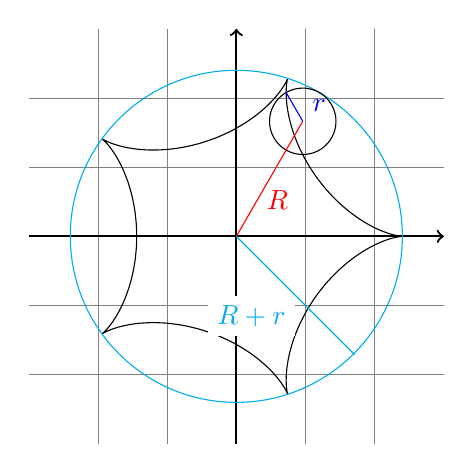
\begin{tikzpicture}[x=0.75pt,y=0.75pt,yscale=1,xscale=1]
            %coordinatum system
            \foreach \i in {-2, ..., 2} {
                \draw [very thin,gray] (\i * 33.33, -100) -- (\i * 33.33, 100);
            }
            \foreach \i in {-2, ..., 2} {
                \draw [very thin,gray] (-100 ,\i * 33.33) -- (100 ,\i * 33.33);
            }
            \draw[thick, ->] (0, -100) -- (0, 100);
            \draw[thick, ->] (-100, 0) -- (100, 0);
            %
            %Hypozykloide
            \draw plot [smooth, variable=\x, domain=0:2*pi, samples = 100] ({64 * cos(\x*180/pi) + 16 * cos(64/16 * \x*180/pi)},{64 * sin(\x*180/pi) - 16 * sin(64/16 * \x*180/pi)});
            %big circle
            \draw [cyan] (0, 0) circle (80);
            \draw [cyan] (0, 0) -- (1.424/4 * 80, -1.424/4 * 80) node[anchor = north east, cyan, fill=white] {$R+r$} -- (1.424/2 * 80, -1.424/2 * 80);
            %small circle (T = pi/3)
            \draw ({64 * cos(60)}, {64 * sin(60)}) circle (16);
            %R
            \draw [red] (0, 0) -- ({20 * cos(60)}, {20 * sin(60)}) node[anchor = west, red] {$R$} -- ({64 * cos(60)}, {64 * sin(60)});
            %r
            \draw [blue] ({64 * cos(60)}, {64 * sin(60)}) node[anchor = south west, blue] {$r$} -- ({64 * cos(60) + 16 * cos(64/16 * 60)},{64 * sin(60) - 16 * sin(64/16 * 60)});
            %
        \end{tikzpicture}\\
    \end{center}

    \subsubsection{Lissajous-Figuren}
    \vspace{0.5em}
    \mathbox{
        \overrightarrow{r}(t) = \binom{a_1 sin(\omega_1 t + \varphi_1)}{a_2 sin(\omega_2 t + \varphi_2)}
    }
    \subsection{Häufige Funktionsgraphen}
    \centerline{
        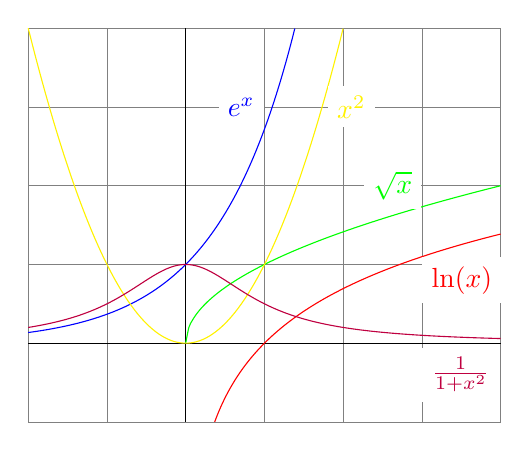
\begin{tikzpicture}
            \draw [help lines] (-2,-1) grid [step=1] (4,4);
            \draw (-2,0) -- (4,0);
            \draw (0,-1) -- (0,4);
            \draw [color = red] plot [smooth, samples = 100, domain = 0.368:4] (\x, {ln(\x)});
                \draw (3, 0.8) node[right, red, fill=white] {$\ln(x)$};
            \draw [color = blue] plot [smooth, samples = 100, domain = -2:1.386] (\x, {e^\x});
                \draw (1,3) node[left, blue, fill=white] {$e^x$};
            \draw [color = green] plot [smooth, samples = 100, domain = 0:4] (\x, {sqrt(\x)});
                \draw (3,2) node[left, green, fill=white] {$\sqrt{x}$};
            \draw [color = yellow] plot [smooth, samples = 100, domain = -2:2] (\x, {(\x)^2});
                \draw (1.8, 3) node[right, yellow, fill=white] {$x^2$};
            \draw [color = purple] plot [smooth, samples = 100, domain = -2:4] (\x, {1/(1+(\x)^2)});
                \draw (3,-0.4
                ) node[right, purple, fill=white] {$\frac{1}{1+x^2}$};
        \end{tikzpicture}
    }
   
\end{document}